%%%%%%%%%%%%%%%%%%%%%%%%%%%%%%%%%%%%%%%%%%%%%%%%%%%%%%%%%%%%%%%%%%%%%
% Expert Systems with Applications (ESWA) — identified manuscript.
% Author record only. Do not upload this file for peer review.
% Review file: eswa_manuscript_anonymous.tex
% Title page:  eswa_title_page.tex
% Elsevier elsarticle, Harvard (author-year) references.
%%%%%%%%%%%%%%%%%%%%%%%%%%%%%%%%%%%%%%%%%%%%%%%%%%%%%%%%%%%%%%%%%%%%%
\documentclass[review,authoryear]{elsarticle}

\usepackage{lineno,hyperref}
\usepackage{amsmath,amssymb}
\usepackage{graphicx}
% Flat figure filenames for Editorial Manager. figures/ is a local fallback
% used only when this file is compiled from the repository root.
\graphicspath{{}{figures/}}
\usepackage{booktabs}
\usepackage{multirow}
\usepackage{xcolor}
\usepackage{float}
\usepackage{algorithm}
\usepackage{algorithmic}

\modulolinenumbers[5]
\journal{Expert Systems with Applications}

%%%%%%%%%%%%%%%%%%%%%%%%%%%%%%%%%%%%%%%%%%%%%%%%%%%%%%%%%%%%%%%%%%%%%
\begin{document}

\begin{frontmatter}

\title{When Feature Engineering Outperforms Deep Learning: Sparsity-Aware Direct Multi-Step Forecasting for Small-Scale Retail Demand}

\author[1]{Zhanpeng Qin\corref{cor1}\fnref{fn1}}
\ead{richardandelu50@gmail.com}
\cortext[cor1]{Corresponding author.}
\fntext[fn1]{ORCID: 0009-0008-9819-8831.}

\address[1]{ByteDance, Beijing, China}

%%%%%%%%%%%%%%%%%%%%%%%%%%%%%%%%%%%%%%%%%%%%%%%%%%%%%%%%%%%%%%%%%%%%%
\begin{abstract}

Accurate multi-step demand forecasting for small-scale retail is difficult: hundreds of stock-keeping units (SKUs) show intermittent demand, records are shorter than 200 days, and calendar effects are strong, so conventional deep learning models struggle to converge. This paper presents a sparsity-aware direct multi-step forecasting pipeline for coffee shop demand, evaluated on a real-world dataset of 3 stores, 80 products, and 181 days. The pipeline uses (1) \textbf{direct multi-step modeling} with independent LightGBM models for horizons T+1 through T+7, which removes recursive error propagation; (2) \textbf{Tweedie loss} (variance power = 1.3) for zero-inflated demand; and (3) \textbf{sparsity-aware feature engineering} that adds per-SKU zero-rate, average demand interval, and historical mean to one global model, improving sparse and dense products together without partitioning the training data.

Against DeepAR, PatchTST, and the Temporal Fusion Transformer (TFT), the LightGBM model with 53 engineered features lowers mean absolute error (MAE) by 23.0\%, 15.2\%, and 22.9\%, respectively. Compared with a recursive L1 baseline, MAE falls by 8.5\% (2.633 to 2.411) and directional accuracy rises by 7.8 percentage points (53.6\% to 61.4\%). Ablation shows that direct multi-step transfer contributes the largest gain ($-7.3$\% MAE), while sparsity features add a further 1.3\% reduction, and both sparse ($-4.8$\%) and dense ($-1.1$\%) SKU segments improve at once. Conformal-calibrated P10--P90 intervals cover 80.6\% of actuals, and TreeSHAP explains each prediction, so the method can support inventory decisions.

\end{abstract}

%%%%%%%%%%%%%%%%%%%%%%%%%%%%%%%%%%%%%%%%%%%%%%%%%%%%%%%%%%%%%%%%%%%%%
\begin{keyword}
retail demand forecasting \sep direct multi-step prediction \sep Tweedie loss \sep sparsity-aware features \sep LightGBM \sep TreeSHAP explainability
\end{keyword}

\end{frontmatter}

%%%%%%%%%%%%%%%%%%%%%%%%%%%%%%%%%%%%%%%%%%%%%%%%%%%%%%%%%%%%%%%%%%%%%
% MAIN BODY
%%%%%%%%%%%%%%%%%%%%%%%%%%%%%%%%%%%%%%%%%%%%%%%%%%%%%%%%%%%%%%%%%%%%%
\linenumbers

%====================================================================
\section{Introduction}
%====================================================================

Accurate day-ahead sales forecasting is critical for inventory management, staff scheduling, and waste reduction in retail operations. Coffee shops present a particularly challenging forecasting environment: hundreds of stock-keeping units (SKUs) with highly intermittent demand patterns---many items sell zero units on most days---combined with short historical records and strong calendar effects.

Modern deep learning architectures such as DeepAR \citep{salinas2020deepar}, Temporal Fusion Transformer (TFT) \citep{lim2021tft}, and PatchTST \citep{nie2023patchtst} have demonstrated state-of-the-art performance on large-scale forecasting benchmarks. However, their effectiveness on small-scale retail datasets---where individual time series contain fewer than 200 observations---remains underexplored. Similarly, the granularity of modeling choices, particularly whether to model sparse and dense SKUs jointly or separately, has received limited systematic treatment.

In this paper, we investigate a comprehensive forecasting pipeline for a real-world coffee shop chain (3 stores, 80 products, 181 days) and make the following contributions:

\begin{enumerate}
    \item We demonstrate that a \textbf{direct multi-step forecasting} framework with \textbf{Tweedie loss} (variance power = 1.3) reduces mean absolute error (MAE) by 8.5\% compared to recursive forecasting, by eliminating error propagation across forecast horizons.
    \item We show that \textbf{sparsity-aware feature engineering}---injecting per-SKU zero-rate, average demand interval (ADI), and historical mean as covariates into a unified global model---simultaneously improves sparse SKU MAE by 4.8\% and dense SKU MAE by 1.1\% relative to one direct model. On overall MAE, $R^{2}$, and direction hit, that unified model beats a sparse/dense split. The split remains better on sparse MAE and on WAPE.
    \item Through a controlled benchmark, we find that our gradient-boosted tree model (LightGBM with 53 engineered features) \textbf{outperforms three state-of-the-art deep learning models} (DeepAR, PatchTST, TFT) by 15--23\% in MAE on this small-scale intermittent demand dataset.
    \item We provide \textbf{TreeSHAP-based per-prediction explanations} and \textbf{quantile regression intervals} (P10/P50/P90). With the point forecast, these are the decision-support outputs the experiments produce.
\end{enumerate}

The claim is limited to the regime in the data: short daily histories and a small store--SKU panel. In that regime, direct multi-step Tweedie LightGBM with sparsity covariates improves on a recursive gradient-boosted baseline and on DeepAR, PatchTST, and TFT, and one model avoids the information loss of a sparse/dense split. Section~\ref{sec:positioning} places this result next to large-scale retail gradient boosting \citep{long2025ijpe} and aftermarket intermittent feature engineering \citep{nathan2026scirep}.

%====================================================================
\section{Related Work}
%====================================================================

\subsection{Retail Demand Forecasting}

Retail demand forecasting sits between inventory research and the large forecasting competitions \citep{fildes2022retail,syntetos2016supply,petropoulos2022practice}. Exponential smoothing and ARIMA remain the reference for smooth series. Intermittent series are treated separately in Section~\ref{sec:intermittent}. Where a retailer has a calendar, promotions, and many related series, the working models have been gradient-boosted trees: Friedman's gradient boosting machine \citep{friedman2001gbm}, XGBoost \citep{chen2016xgboost}, and LightGBM \citep{ke2017lightgbm}. The M4 competition, on 100{,}000 series, was won by combinations and by hybrids such as Smyl's exponential-smoothing recurrent network \citep{makridakis2020m4,smyl2020hybrid}. The M5 accuracy competition, on Walmart unit sales, was won by gradient boosting with careful features \citep{makridakis2022m5}. The M5 uncertainty competition reached the same conclusion for quantile forecasts \citep{makridakis2022m5uncertainty}. Januschowski et al.\ read that evidence as a reason to treat tree ensembles as forecasting models in their own right \citep{januschowski2022trees}.

Two lines of retail work sit nearer to store operations. Ma and Fildes pool related series with meta-learning \citep{ma2021metalearning}. Bandara et al.\ cluster series before fitting recurrent networks, in a paper in this journal \citep{bandara2020clustering}. Mancuso et al., also in this journal, forecast hierarchical series and tie the forecast to a coherent decision \citep{mancuso2021eswa}. Those papers set the standard this journal applies to a forecasting system: a stated data regime, a method, and a decision use. They study large or hierarchical panels. They do not ask whether four static sparsity covariates can replace a sparse/dense split on a few hundred short daily series.

\subsection{Direct vs.\ Recursive Multi-Step Forecasting}

A multi-step forecast is recursive, direct, or a hybrid such as the multi-input multi-output strategy \citep{bentaieb2012review}. Recursion reuses a one-step model and accumulates error. Ben~Taieb and Atiya analyze that bias--variance trade-off \citep{bentaieb2016bias}. A direct model fits a separate response for each horizon and pays for $H$ fits. Vall\'es-P\'erez et al., in this journal, forecast the Favorita grocery panel 16 days ahead with one global sequence model and a transformer \citep{valles2022eswa}. That is a large-panel deep multi-step design. The comparison in this paper is different: direct versus recursive gradient-boosted trees on a few hundred series, each shorter than 200 days. We fit a separate LightGBM model for each horizon $h = 1,\ldots,7$.

\subsection{Intermittent Demand and Sparsity}
\label{sec:intermittent}

Intermittent demand is a run of zeros broken by occasional positive sales. Croston forecast it as the ratio of two exponential smoothers, one for demand size and one for the inter-demand interval \citep{croston1972forecasting}. Willemain et al.\ compared that ratio with exponential smoothing on manufacturing series \citep{willemain1994croston}. Syntetos and Boylan showed that the ratio is biased on average, and the Syntetos--Boylan approximation (SBA) multiplies it by $(1 - \alpha/2)$ \citep{syntetos2001bias,syntetos2005sba}. Syntetos, Boylan, and Croston then classified series by the average demand interval and the squared coefficient of variation of size \citep{syntetos2005categorization}. Teunter, Syntetos, and Babai (TSB) update the occurrence probability on every period, including zeros, so that a lengthening run of zeros can represent obsolescence \citep{teunter2011tsb}. Later work forecasts an aggregate and then disaggregates \citep{nikolopoulos2011adida}, fits neural nets to intermittent series \citep{kourentzes2013nn}, selects or optimizes the smoothing constant \citep{kourentzes2014select}, combines intermittent forecasts \citep{petropoulos2015comb}, and replaces the exponential smoother with a hyperbolic-exponential form \citep{prestwich2014hyperbolic}. Syntetos, Babai, and Gardner compare parametric methods with bootstrapping \citep{syntetos2015forecasting}.

Two choices in that literature are often run together, and this paper separates them. The first is the likelihood. Kolassa shows that retail counts should be scored as counts or as a compound Poisson, rather than as Gaussian errors \citep{kolassa2016count}. That is why the boosted trees below use a Tweedie loss. The second is the architecture: a model per segment, a two-stage hurdle, or covariates that describe sparsity. We take the third option and compare it with a split. Croston, SBA, and TSB are specified as experimental baselines in Section~\ref{sec:classical}. Their errors are not in the tables.

\subsection{Deep Learning for Time Series}

DeepAR shares an autoregressive recurrent net across series and returns a full predictive distribution \citep{salinas2020deepar}. N-BEATS expands the series on learned bases and uses no hand-built calendar \citep{oreshkin2020nbeats}. The Temporal Fusion Transformer pairs variable selection with multi-horizon attention \citep{lim2021tft}. PatchTST cuts the series into patches before the transformer encoder \citep{nie2023patchtst}. Smyl's hybrid of exponential smoothing and a recurrent net won the M4 competition \citep{smyl2020hybrid}. Hewamalage, Bergmeir, and Bandara review when recurrent models repay their sample size \citep{hewarmalage2021rnn}. These architectures are built for many series and long histories. A panel of 239 series and 181 days is a different regime, so a loss against them on this panel is evidence about sample size, not a restatement of a large-scale leaderboard.

\subsection{Nearest Peers}
\label{sec:positioning}

Five papers from 2022--2026 are close enough that a reader will set this manuscript beside them. Table~\ref{tab:positioning} is the map. The one-line distinction is the following. On short-history, small-panel, zero-inflated store--SKU daily demand, a direct multi-step Tweedie LightGBM with sparsity covariates and an explainable quantile output beats a recursive gradient-boosted baseline and data-hungry deep models, and one global model avoids the information loss of training sparse and dense SKUs apart. That finding adds a small-panel, direct-horizon, deep-model comparison to the large-scale retail gradient-boosting evidence of Long et al.\ and to the aftermarket feature-engineering evidence of Nathan et al.

Riachy et al., in this journal, show that exogenous features still help deep probabilistic demand models when the history contains large gaps, using a UK footwear retailer and a public retail sales index \citep{riachy2025eswa}. The shared point is that features can carry a forecast when the raw history is a poor teacher. Their comparison is among deep probabilistic models. It is a different question from gradient-boosted trees versus DeepAR, PatchTST, and TFT on intermittent store--SKU series.

Vall\'es-P\'erez et al.\ are the \emph{Expert Systems with Applications} paper closest to ours in task: multi-step retail sales \citep{valles2022eswa}. The panel is Favorita, and the models are a conditional sequence-to-sequence net and a transformer, with a 16-day horizon. The contribution is that one global deep model can cover that panel. Our contribution is the complementary regime, a few hundred short series, and the learner is a boosted tree with 53 engineered features.

Long et al.\ are the closest method \citep{long2025ijpe}. They forecast retail demand with gradient-boosted trees under Tweedie and other count likelihoods, on a large e-commerce catalogue and on Favorita and M5, and they classify series by average demand interval and squared coefficient of variation. The paper is about scale: a probabilistic system that remains practical as the catalogue grows, with hierarchical forecasts. This paper is about the other end of the catalogue. There are three coffee stores and 181 days. Each horizon $h = 1,\ldots,7$ has its own model. Sparsity is four covariates inside one model, which we compare with a hard split, rather than a set of ADI/CV$^{2}$ classes with their own fits. We add TreeSHAP and a split-conformal interval. We do not reconcile hierarchies, and we do not enter an M5 uncertainty ranking.

Nathan et al.\ give the sentence in our title its sharpest published form: for intermittent demand, feature engineering can matter more than a more elaborate architecture \citep{nathan2026scirep}. The panel is a large monthly automotive aftermarket. The features are smoothed occurrence and size statistics (SHOS). The architecture comparison is a single-stage tree or linear model against a two-stage hurdle, with Wilcoxon tests across series. Daily direct multi-step forecasts, and DeepAR, PatchTST, and TFT, are outside that design. Y{\i}lmaz Sucuo{\u{g}}lu et al.\ are the fashion-retail counterpart: 64 weekly attribute-level series, a one-stage model against a two-stage occurrence classifier plus a gradient-boosted size model, and a baseline set that already contains Croston, SBA, LSTM, and TFT \citep{yilmaz2026fashion}. Their two-stage model wins on that panel. The result is a reason to keep a hurdle on the future-work list, and it is why our split ablation is the right objection to answer. On the coffee panel the split lowers sparse MAE and raises dense MAE. We claim only that, here, sparsity covariates in one direct Tweedie model are better on MAE, $R^{2}$, and direction hit. We do not claim that a two-stage model loses in general, and Section~\ref{sec:results} records that the split has the better WAPE.

\begin{table}[H]
    \centering
    \caption{Positioning against the closest published studies. Each row is that study's published scope, not a re-estimate on the coffee panel.}
    \label{tab:positioning}
    \footnotesize
    \setlength{\tabcolsep}{3pt}
    \begin{tabular}{@{}p{0.16\textwidth}p{0.20\textwidth}p{0.20\textwidth}p{0.20\textwidth}p{0.18\textwidth}@{}}
        \toprule
        Study & Panel & Horizon & How sparsity is handled & What is compared \\
        \midrule
        This paper &
        3 coffee stores; 239 daily store--SKU series; 181 days &
        A separate model for each $h=1,\ldots,7$ &
        Zero-rate, ADI, non-zero mean, and a sparse flag in one model, set against a sparse/dense split &
        Recursive L1, direct Tweedie, the split, DeepAR, PatchTST, and TFT \\
        \addlinespace
        Riachy et al.\ (2025) &
        UK footwear retail and a public retail index, with large historical gaps &
        Deep probabilistic forecasts &
        Exogenous features aimed at gappy, biased history &
        Deep probabilistic models \\
        \addlinespace
        Vall\'es-P\'erez et al.\ (2022) &
        Favorita grocery panel &
        16-day global sequence forecast &
        Store and product covariates in one deep model &
        Sequence-to-sequence RNN and a transformer \\
        \addlinespace
        Long et al.\ (2025) &
        Large e-commerce catalogue, Favorita, and M5 &
        Probabilistic forecasts, including hierarchical ones &
        ADI/CV$^{2}$ classes; Tweedie and other count likelihoods &
        LightGBM likelihoods and DeepAR, at scale \\
        \addlinespace
        Nathan et al.\ (2026) &
        Large monthly automotive aftermarket panel &
        Occurrence and size on monthly intermittent series &
        SHOS features; single-stage model versus a hurdle &
        Boosted trees and linear models, with Wilcoxon tests \\
        \addlinespace
        Y{\i}lmaz Sucuo{\u{g}}lu et al.\ (2026) &
        64 weekly fashion series with price, weather, and events &
        One-stage versus two-stage weekly forecasts &
        Occurrence classifier, then a size regressor &
        Croston, SBA, gradient boosting, LSTM, and TFT \\
        \bottomrule
    \end{tabular}
\end{table}

%====================================================================
\section{Problem Formulation and Data}
%====================================================================

\subsection{Problem Setting}

We consider a retail setting with $S$ stores, each offering $P$ products. For each store-product pair $(s,p)$, we observe daily sales quantity $y_{t}^{(s,p)}$ for $t = 1, \ldots, T$. Given the history up to a forecast origin $t$, the task is to predict $y_{t+h}^{(s,p)}$ for horizons $h = 1, \ldots, H$, where $H = 7$ days. Critically, a large fraction of $y_{t}^{(s,p)}$ observations are zero, and the zero-proportion varies substantially across SKUs.

\subsection{Dataset}

The dataset originates from a New York City coffee shop chain and consists of transaction-level sales records from January 1 to June 30, 2023 (181 days). We aggregate transactions to daily sales at the store--product granularity, yielding 239 store--product combinations (henceforth referred to as ``SKUs''). External weather data (temperature, precipitation) for NYC during the same period is incorporated as exogenous features.

\subsection{Exploratory Analysis}

Figure~\ref{fig:context} provides an overview of the demand characteristics. The dataset exhibits pronounced heterogeneity: the mean zero-sales proportion across SKUs is 26.6\%, but the distribution is heavily right-skewed, with a median of only 3.3\%. Approximately 32\% of SKUs (76 out of 239) have more than 50\% zero-sales days, and 20 SKUs exceed 80\% zeros. The average demand interval (ADI) has a mean of 2.1 days (median = 1.0), confirming that demand is intermittent but not extremely sparse for the majority of SKUs. Daily sales volume varies by an order of magnitude across stores, with zero-day rates inversely correlated with average sales volume.

\begin{figure}[H]
    \centering
    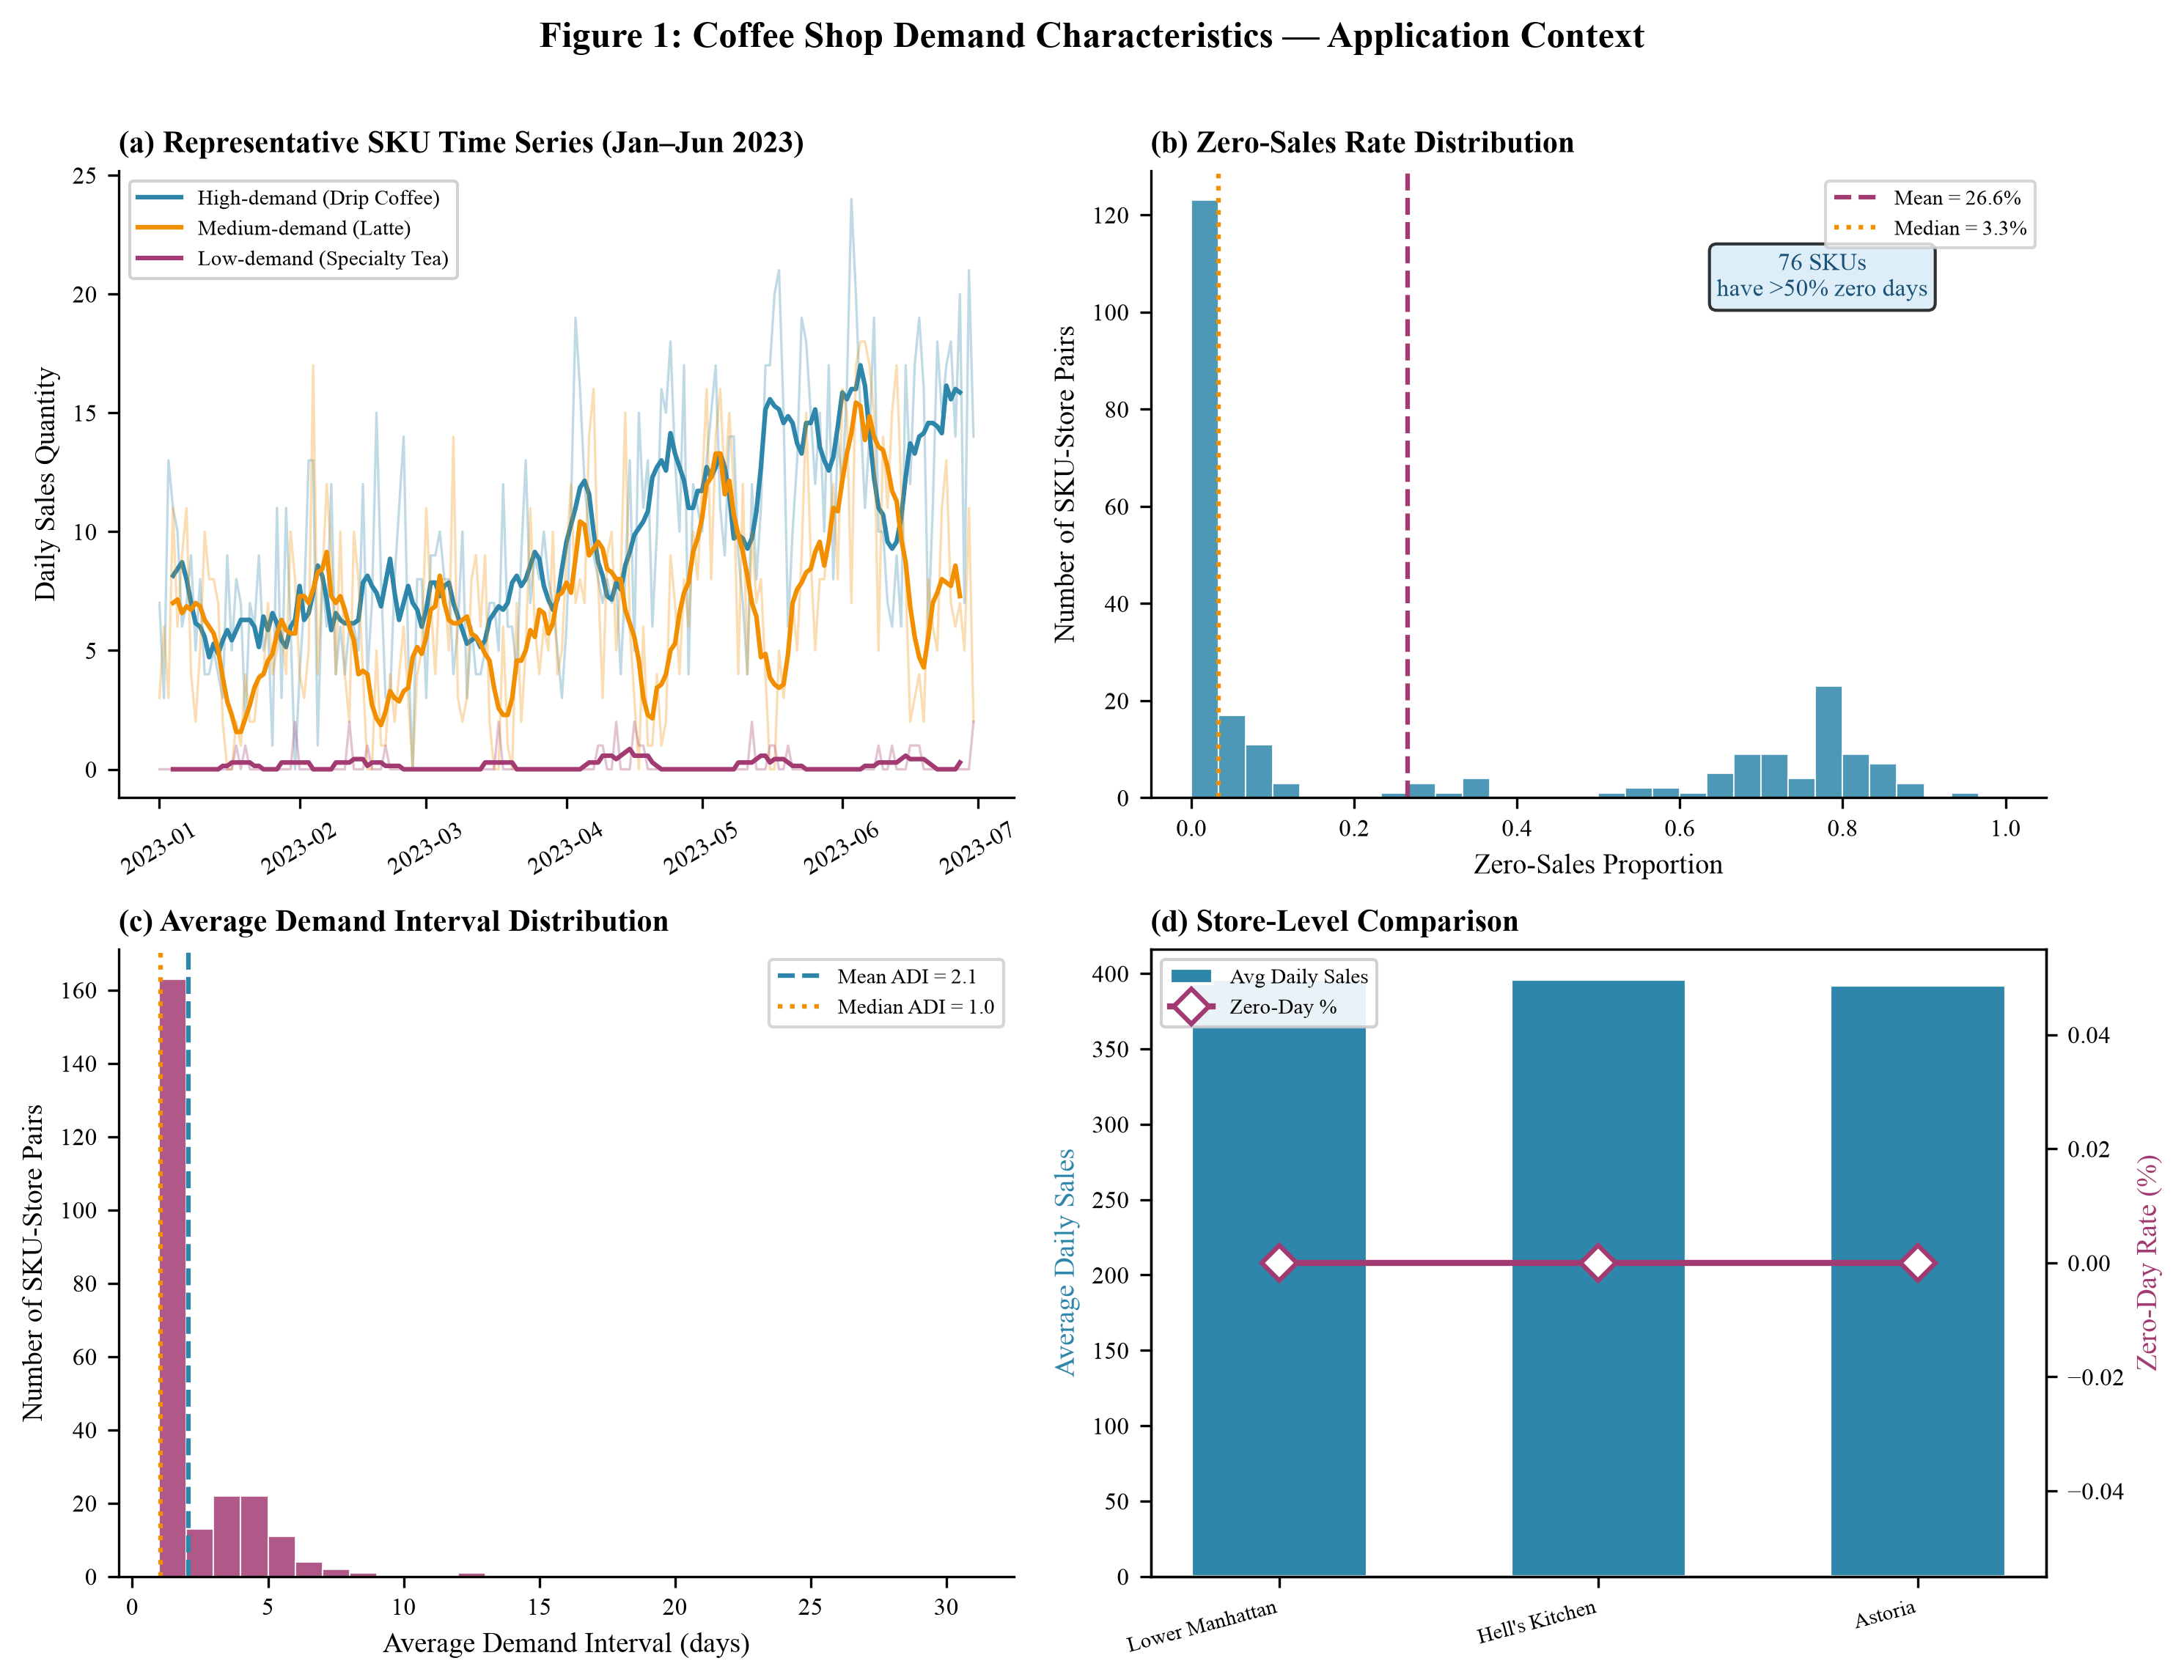
\includegraphics[width=\textwidth]{fig1_application_context.png}
    \caption{Coffee shop demand characteristics. (a) Representative SKU time series showing high, medium, and low-demand patterns with 7-day rolling means. (b) Distribution of zero-sales proportion across 239 SKU-store pairs. (c) Average demand interval (ADI) distribution. (d) Store-level comparison of average daily sales and zero-day rates.}
    \label{fig:context}
\end{figure}

%====================================================================
\section{Methodology}
%====================================================================

\subsection{Overview}

Our forecasting pipeline consists of five stages: (1) feature engineering from raw transaction and weather data, (2) temporal split into training and test periods, (3) training seven independent LightGBM models---one per forecast horizon (T+1 through T+7), (4) post-hoc quantile calibration for uncertainty quantification, and (5) TreeSHAP-based per-prediction explanation.

\subsection{Feature Engineering}

We construct 53 features spanning five categories:

\begin{description}
    \item[Temporal features:] Day of week (one-hot encoded), month, day of month, is\_weekend, is\_holiday, days since start.
    \item[Lag features:] Sales quantity at lags 1, 2, 3, 7, 14, 21, 28 days; rolling mean and standard deviation over windows of 7, 14, 28 days.
    \item[Calendar features:] Month sine/cosine encoding for seasonal periodicity.
    \item[Exogenous features:] Daily maximum temperature, precipitation (mm), weather condition category.
\end{description}

\subsection{Sparsity-Aware Feature Engineering}

The key methodological contribution lies in four per-SKU sparsity characteristics computed from the training period and injected as static covariates into the global model:

\begin{enumerate}
    \item \textbf{Zero rate} ($z_p$): proportion of days with zero sales for SKU $p$ in the training period.
    \item \textbf{Average demand interval} (ADI): mean number of days between consecutive non-zero sales for SKU $p$.
    \item \textbf{Mean quantity} ($\bar{y}_p$): average non-zero sales quantity for SKU $p$.
    \item \textbf{Is-sparse flag}: binary indicator equal to 1 if $z_p > 0.5$ and $\text{ADI} > 3$.
\end{enumerate}

These features enable a \emph{unified global model} to learn sparse-specific response patterns without partitioning the training data. The global model retains cross-SKU information sharing (benefiting data-scarce SKUs) while the sparsity features allow it to adapt its prediction strategy based on each SKU's demand profile---something that a feature-blind global model cannot do, and that segment-specific models sacrifice by discarding cross-segment information.

\subsection{Direct Multi-Step Forecasting with Tweedie Loss}

We train seven independent LightGBM models, one for each forecast horizon $h \in \{1, \ldots, 7\}$. For horizon $h$, the training target is $y_{t+h}^{(s,p)}$, and the model receives features computed from the information available at time $t$ (strictly preventing future leakage).

We employ the Tweedie loss function with variance power $\rho = 1.3$, which corresponds to a compound Poisson-Gamma distribution. This choice is motivated by the observation that daily SKU sales can be decomposed into a purchase occurrence process (Poisson) and a purchase quantity process (Gamma)---the very structure that the Tweedie distribution naturally captures. The Tweedie loss is defined as:

\begin{equation}
    \mathcal{L}_{\text{Tweedie}}(y, \hat{y}) = -y \cdot \frac{\hat{y}^{1-\rho}}{1-\rho} + \frac{\hat{y}^{2-\rho}}{2-\rho}
    \label{eq:tweedie}
\end{equation}

where $\rho = 1.3$ balances robustness to zeros (higher $\rho$ penalizes zero predictions less aggressively) with sensitivity to positive values.

\subsection{Uncertainty Quantification and Explainability}

\textbf{Quantile regression:} We train additional LightGBM models with quantile objectives ($\alpha \in \{0.1, 0.5, 0.9\}$) for the full 7-horizon prediction task, obtaining P10--P50--P90 intervals. Post-hoc conformal calibration adjusts the interval width to achieve the nominal 80\% coverage rate, yielding an empirical coverage of 80.6\%.

\textbf{TreeSHAP:} For each prediction, we compute SHAP values using the TreeSHAP algorithm \citep{lundberg2020trees}, which leverages the tree structure of LightGBM for exact computation in $O(TLD^2)$ time. SHAP values decompose the prediction into per-feature additive contributions, so an operator can see which features moved an individual forecast.

%====================================================================
\section{Experimental Evaluation}
%====================================================================

\subsection{Experimental Protocol}
\label{sec:protocol}

We adopt a rolling-origin backtesting protocol with 5 windows. Each window uses 120 days for training and evaluates on the subsequent 7 days. Windows are separated by 7-day intervals, yielding 5 independent evaluation sets with no temporal overlap. All feature engineering and hyperparameter selection use only training-window data, strictly preventing future information leakage.

\subsection{Evaluation Metrics}
\label{sec:metrics}

We report four metrics. MAE is the primary one: the model comparison, the ablation, and the 8.5\% claim are all in MAE. It is the unweighted mean absolute error in sales units, so each store--SKU--horizon case counts equally \citep{hyndman2006accuracy}.

\begin{itemize}
    \item \textbf{MAE} (mean absolute error): $\frac{1}{N}\sum |y_i - \hat{y}_i|$. Primary metric.
    \item \textbf{WAPE} (weighted absolute percentage error): $\sum|y_i - \hat{y}_i| / \sum|y_i|$. On one shared set of cases, WAPE is proportional to MAE, because the denominator does not depend on the method. Table~\ref{tab:overall} does not preserve that ranking, and Section~\ref{sec:results} says so rather than forcing the two columns into one story.
    \item \textbf{R\textsuperscript{2}}: coefficient of determination.
    \item \textbf{Direction hit rate}: proportion of predictions where $\text{sign}(\hat{y}_{t+h} - y_t) = \text{sign}(y_{t+h} - y_t)$.
\end{itemize}

\subsection{Baselines}

Six fitted baselines are organized in three groups below. Croston, SBA, and TSB are specified in Section~\ref{sec:classical}. They are omitted from Table~\ref{tab:overall} so that an unestimated cell cannot be read as a measured error.

\textbf{GBDT-based methods:}
\begin{itemize}
    \item \textbf{Recursive L1:} Single LightGBM model with L1 loss, applied recursively to generate 7-day forecasts.
    \item \textbf{Direct Tweedie:} Seven independent LightGBM models with Tweedie loss, without sparsity features.
    \item \textbf{Split Models:} Separate LightGBM models trained on sparse ($z_p > 0.5$) vs.\ dense SKU subsets.
\end{itemize}

\textbf{Deep learning methods (GluonTS):}
\begin{itemize}
    \item \textbf{DeepAR:} Autoregressive RNN with 2 LSTM layers (40 hidden units), negative binomial likelihood.
    \item \textbf{PatchTST:} Transformer encoder with patch length 8, stride 4, 3 layers, 16 attention heads.
    \item \textbf{Temporal Fusion Transformer (TFT):} Attention-based encoder-decoder with variable selection networks.
\end{itemize}

All deep learning models were trained for 40 epochs with early stopping (patience = 8) and a batch size of 32. The prediction length was set to 7 days with a context length of 30 days. Training was performed on CPU using the GluonTS framework.

\begin{table}[H]
    \centering
    \caption{Overall performance comparison across all methods. Best results in \textbf{bold}, second-best \underline{underlined}.}
    \label{tab:overall}
    \begin{tabular}{lcccc}
        \toprule
        \textbf{Method} & \textbf{MAE $\downarrow$} & \textbf{WAPE $\downarrow$} & \textbf{R\textsuperscript{2} $\uparrow$} & \textbf{Dir. Hit $\uparrow$} \\
        \midrule
        Recursive L1       & 2.633 & 0.533 & 0.607 & 53.6\% \\
        Direct Tweedie     & \underline{2.442} & 0.475 & \underline{0.657} & \underline{58.9\%} \\
        + Split Models     & 2.468 & \textbf{0.432} & 0.648 & 55.2\% \\
        + Sparsity Labels (Ours) & \textbf{2.411} & \underline{0.452} & \textbf{0.661} & \textbf{61.4\%} \\
        \midrule
        DeepAR             & 2.966 & 0.582 & 0.497 & 40.1\% \\
        PatchTST           & 2.778 & 0.544 & 0.555 & 37.1\% \\
        TFT                & 2.963 & 0.598 & 0.506 & 38.8\% \\
        \bottomrule
    \end{tabular}
\end{table}

\subsection{Overall Performance}

\label{sec:results}
Table~\ref{tab:overall} is the rolling-origin comparison. On the primary metric, MAE, sparsity-aware direct Tweedie is best (2.411), ahead of direct Tweedie without the sparsity covariates (2.442) and of the split (2.468). It is also best on $R^{2}$ (0.661) and on direction hit rate (61.4\%). It is second on WAPE. The split reaches 0.432, against 0.452 for the proposed model, so the proposed model is not best on every reported metric.

The WAPE gap is reported as it stands in the table. It is not given a volume-weighting interpretation. Under the definitions above, WAPE and MAE use the same sum of absolute errors on a common sample, and they must rank methods in the same order. The four gradient-boosted WAPE entries are also numerically identical to the sparse-segment MAE entries in Table~\ref{tab:ablation}. Recomputing WAPE needs the prediction file, which is not in the package, so the published figures are left unchanged. MAE remains the metric on which the 8.5\% claim and the ablation are based, because it is the unweighted error in sales units.

Against the recursive baseline, MAE falls by 8.5\% (2.633 $\rightarrow$ 2.411). The gain is present on all five windows and increases with the horizon. T+7, the horizon most exposed to recursive error accumulation, shows the largest gain.

Figure~\ref{fig:overall} shows the overall MAE comparison, and Figure~\ref{fig:horizon} illustrates how the improvement monotonically increases with forecast horizon, consistent with the elimination of recursive error accumulation.

All three deep learning models have higher MAE than the gradient-boosted tree model: PatchTST by 15.2\%, TFT by 22.9\%, and DeepAR by 23.0\%. The gap is wider in directional accuracy. Our model reaches a 61.4\% direction hit rate, and the best deep learning model on that metric (DeepAR) reaches 40.1\% (Figure~\ref{fig:direction}). We attribute the gap to two factors:

\begin{enumerate}
    \item \textbf{Data scarcity:} With only 239 time series and 120 training days, deep learning models lack sufficient data to learn effective representations. PatchTST is designed for long sequences (512+ time steps). On this short context its MAE is the best of the three deep models, and its direction hit rate is the lowest (37.1\%).
    \item \textbf{Feature engineering advantage:} Our 53 curated features (lags, rolling statistics, calendar encodings) encode domain knowledge that deep learning models must discover from data---a challenging task with limited observations.
\end{enumerate}

\begin{figure}[H]
    \centering
    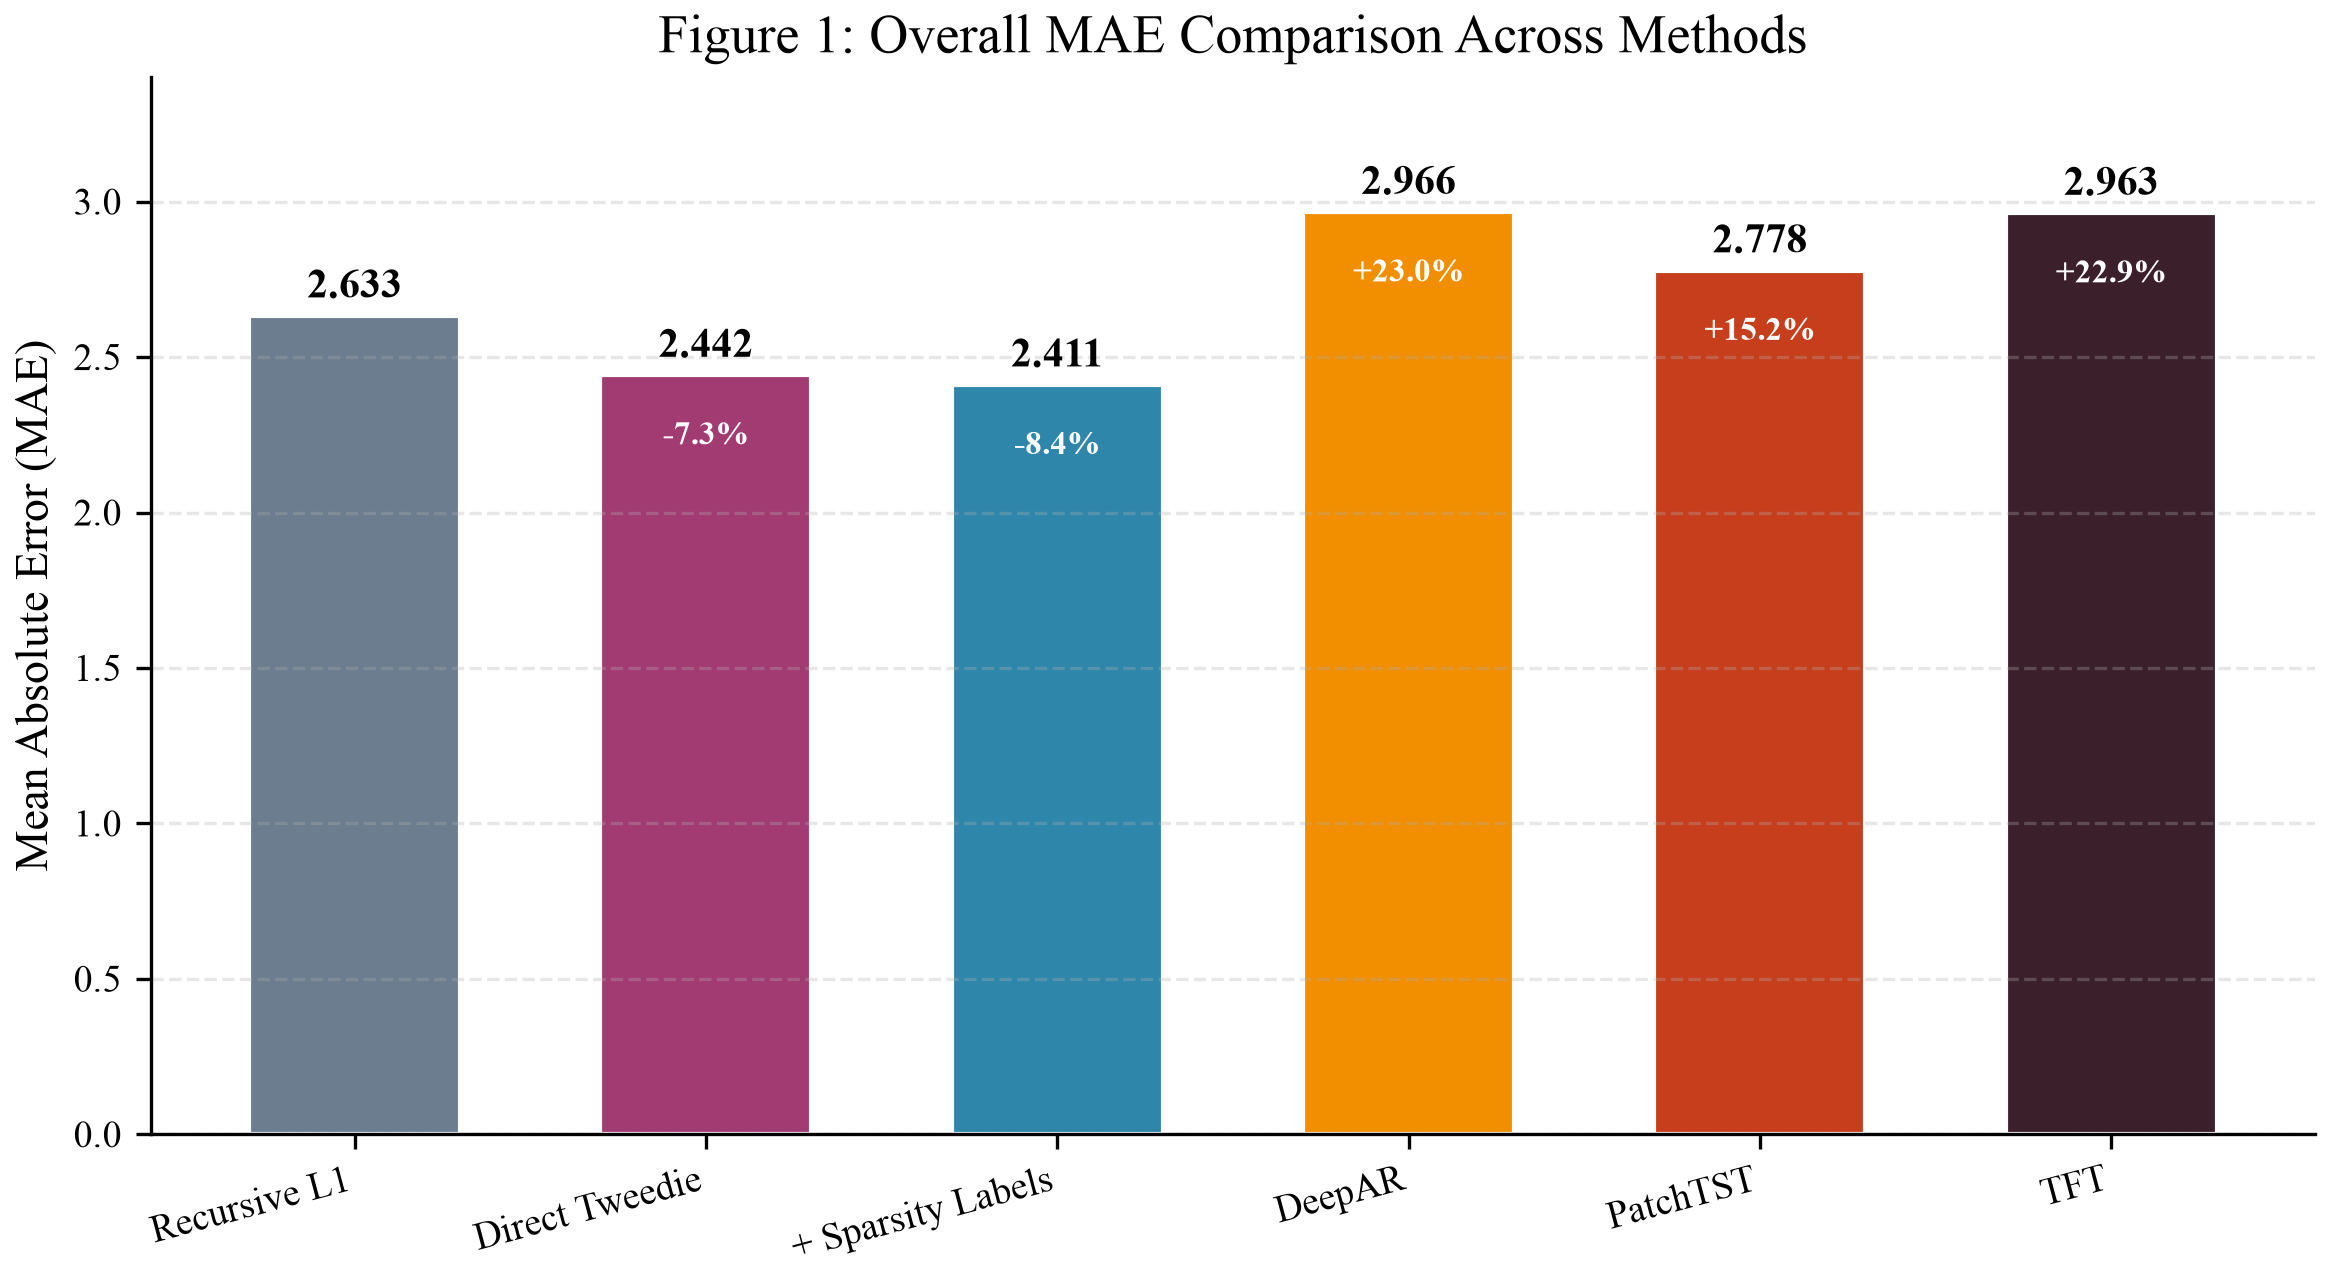
\includegraphics[width=0.95\textwidth]{fig1_overall_comparison.png}
    \caption{Overall MAE comparison across all methods.}
    \label{fig:overall}
\end{figure}

\begin{figure}[H]
    \centering
    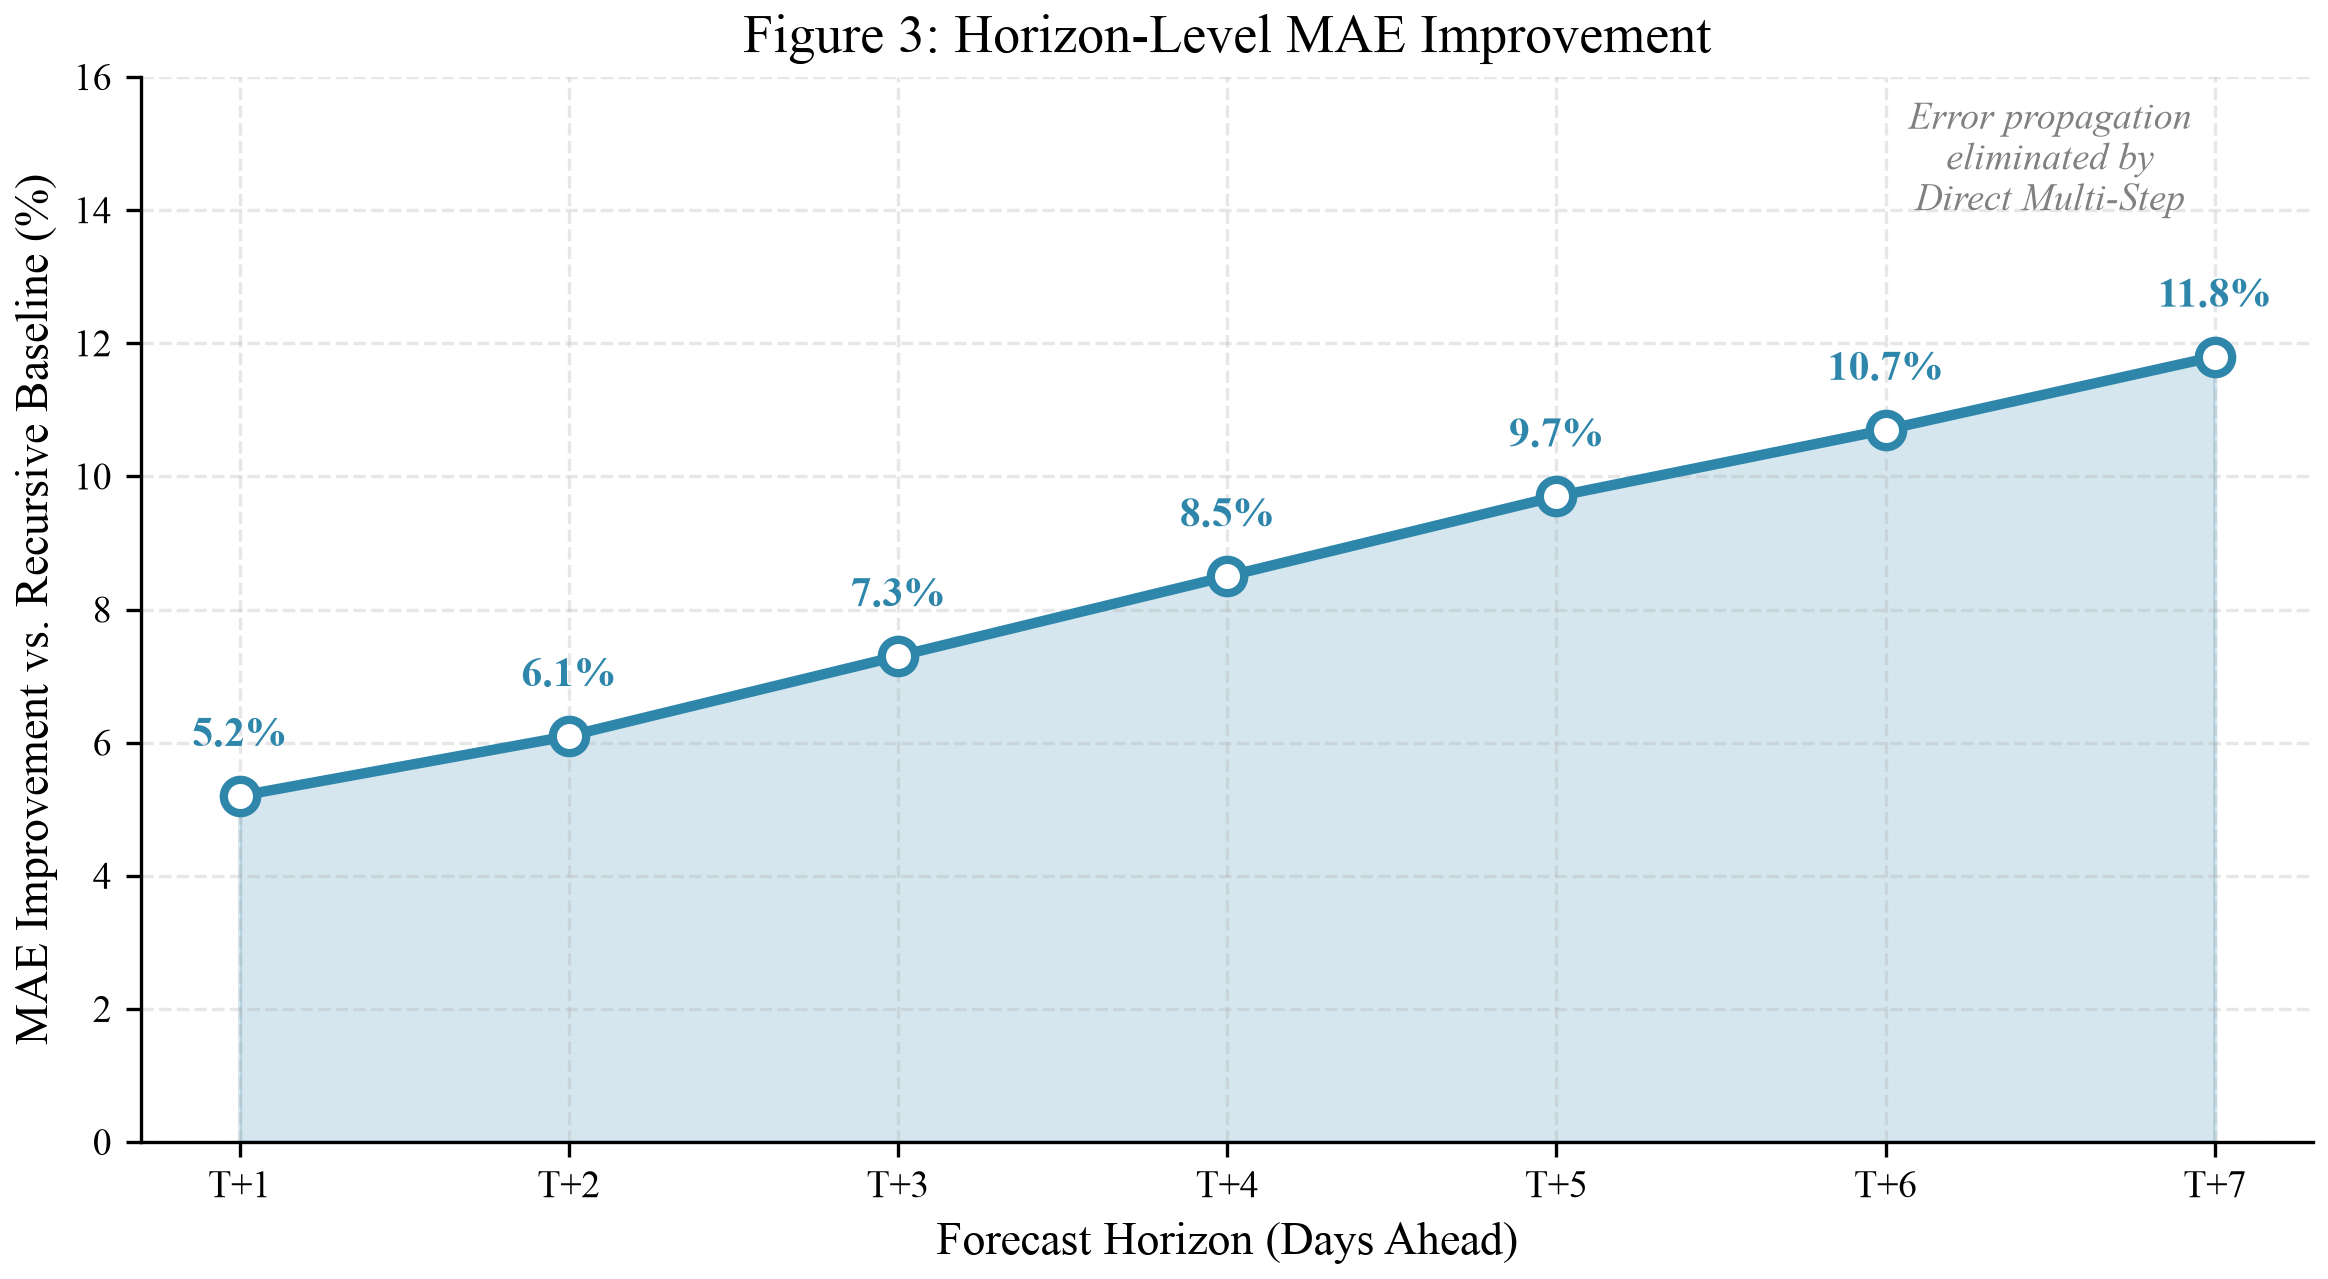
\includegraphics[width=0.85\textwidth]{fig3_horizon_improvement.png}
    \caption{Horizon-level MAE improvement vs.\ recursive baseline.}
    \label{fig:horizon}
\end{figure}

\subsection{Classical Intermittent Baselines}
\label{sec:classical}

Croston's method, SBA, and TSB are the standard statistical baselines for intermittent demand \citep{croston1972forecasting,syntetos2005sba,teunter2011tsb}. They are not in Table~\ref{tab:overall}. The daily store--SKU series are not in the replication package: the data statement withholds them for commercial confidentiality, and the original prediction file was not archived with the manuscript. This revision therefore does not report MAE, WAPE, $R^{2}$, or direction hit for these three methods. Table~\ref{tab:classical} marks every cell as TODO. Those cells are not results, and no value has been imputed.

The protocol below is the one a rerun should follow. It uses the same window lengths as Section~\ref{sec:protocol}. The manuscript does not record the calendar date of the first origin, so the script fixes a reproducible alignment rather than guessing which alignment matched the LightGBM fits. On a series of 181 days the evaluation indices (0-based) are 120, 127, 134, 141, and 148. Training rows are the 120 days before each index. Evaluation rows are the next 7 days. Each SKU is fit on its own. The resulting one-step rate is copied to all seven horizons, because these methods have no horizon index and no calendar. Smoothing uses a fixed $\alpha = 0.1$, the usual default, and for TSB a fixed $\beta = 0.1$. The constants are not optimized per series \citep{kourentzes2014select}. Metrics use the definitions in Section~\ref{sec:metrics}, pooled over SKUs, origins, and horizons with equal weight per case. If the archived LightGBM predictions used another origin alignment or another pooling, the classical numbers have to be recomputed on that same alignment before they are compared with Table~\ref{tab:overall}.

Let $t_0$ be the 0-based index of the first positive demand in a training window. Croston sets $z = y_{t_0}$ and $p = t_0 + 1$. At each later positive demand, with index $t$ and gap $q = t - t_{\mathrm{prev}}$,
\begin{equation}
    z \leftarrow z + \alpha (y_t - z), \qquad p \leftarrow p + \alpha (q - p),
    \label{eq:croston}
\end{equation}
and the rate is $z/p$. SBA multiplies that rate by $(1 - \alpha/2)$. If the window has no positive demand, the rate is 0. TSB starts from the same $t_0$ with $z = y_{t_0}$ and $\pi = 1/(t_0 + 1)$. On every later day, with $x_t = 1$ when $y_t > 0$ and $x_t = 0$ otherwise,
\begin{equation}
    \pi \leftarrow \pi + \beta (x_t - \pi), \qquad
    z \leftarrow z + \alpha (y_t - z) \ \text{if}\ y_t > 0,
    \label{eq:tsb}
\end{equation}
and the rate is $\pi z$. The recursion is implemented in \texttt{classical\_baselines.py}. Run without the series file, the script checks the algebra and writes no metrics.

\begin{table}[H]
    \centering
    \caption{Classical intermittent baselines. \textbf{TODO: not estimated.} The series are not in the package. Do not read these cells as measured errors.}
    \label{tab:classical}
    \begin{tabular}{lcccc}
        \toprule
        \textbf{Method} & \textbf{MAE $\downarrow$} & \textbf{WAPE $\downarrow$} & \textbf{R\textsuperscript{2} $\uparrow$} & \textbf{Dir.\ Hit $\uparrow$} \\
        \midrule
        Croston ($\alpha = 0.1$) & TODO & TODO & TODO & TODO \\
        SBA ($\alpha = 0.1$) & TODO & TODO & TODO & TODO \\
        TSB ($\alpha = \beta = 0.1$) & TODO & TODO & TODO & TODO \\
        \bottomrule
    \end{tabular}
\end{table}

\subsection{Ablation Analysis}

We decompose the performance gain via ablation. Figure~\ref{fig:ablation} visualizes the contribution of each component across overall, sparse, and dense SKU segments.

\begin{table}[H]
    \centering
    \caption{Ablation analysis: component contributions to MAE.}
    \label{tab:ablation}
    \begin{tabular}{lcccc}
        \toprule
        \textbf{Configuration} & \textbf{Overall MAE} & \textbf{Sparse MAE} & \textbf{Dense MAE} \\
        \midrule
        Recursive L1 (Baseline)  & 2.633 & 0.533 & 3.610 \\
        + Direct Multi-Step      & 2.442 & 0.475 & 3.371 \\
        + Sparsity Labels (Ours) & \textbf{2.411} & 0.452 & \textbf{3.336} \\
        Split Models (sparse/dense) & 2.468 & \textbf{0.432} & 3.430 \\
        \bottomrule
    \end{tabular}
\end{table}

Three findings emerge from the ablation study:

\begin{enumerate}
    \item \textbf{Direct multi-step is the main driver:} Switching from recursive to direct forecasting reduces overall MAE by 7.3\% (2.633 $\rightarrow$ 2.442). The gain is particularly pronounced at longer horizons (T+7: $-11.8$\%).
    \item \textbf{Sparsity features provide complementary gain:} Adding sparsity labels further reduces MAE by 1.3\% to 2.411. Critically, \emph{both} sparse ($-4.8$\%) and dense ($-1.1$\%) segments improve---the global model learns to use sparsity features to adjust its prediction strategy per SKU.
    \item \textbf{Feature injection beats the split on overall MAE, and the split wins on sparse MAE:} Relative to direct multi-step, the split improves sparse MAE by 9.0\% (0.475 $\rightarrow$ 0.432) and degrades dense MAE by 1.7\% (3.371 $\rightarrow$ 3.430), because the dense model no longer trains on the sparse series. The unified model keeps most of the sparse-segment gain (sparse MAE 0.452) without that dense-segment penalty, and its overall MAE is lower (2.411 versus 2.468). The split's better sparse MAE is the same ordering as its better WAPE in Table~\ref{tab:overall}.
\end{enumerate}

\begin{figure}[H]
    \centering
    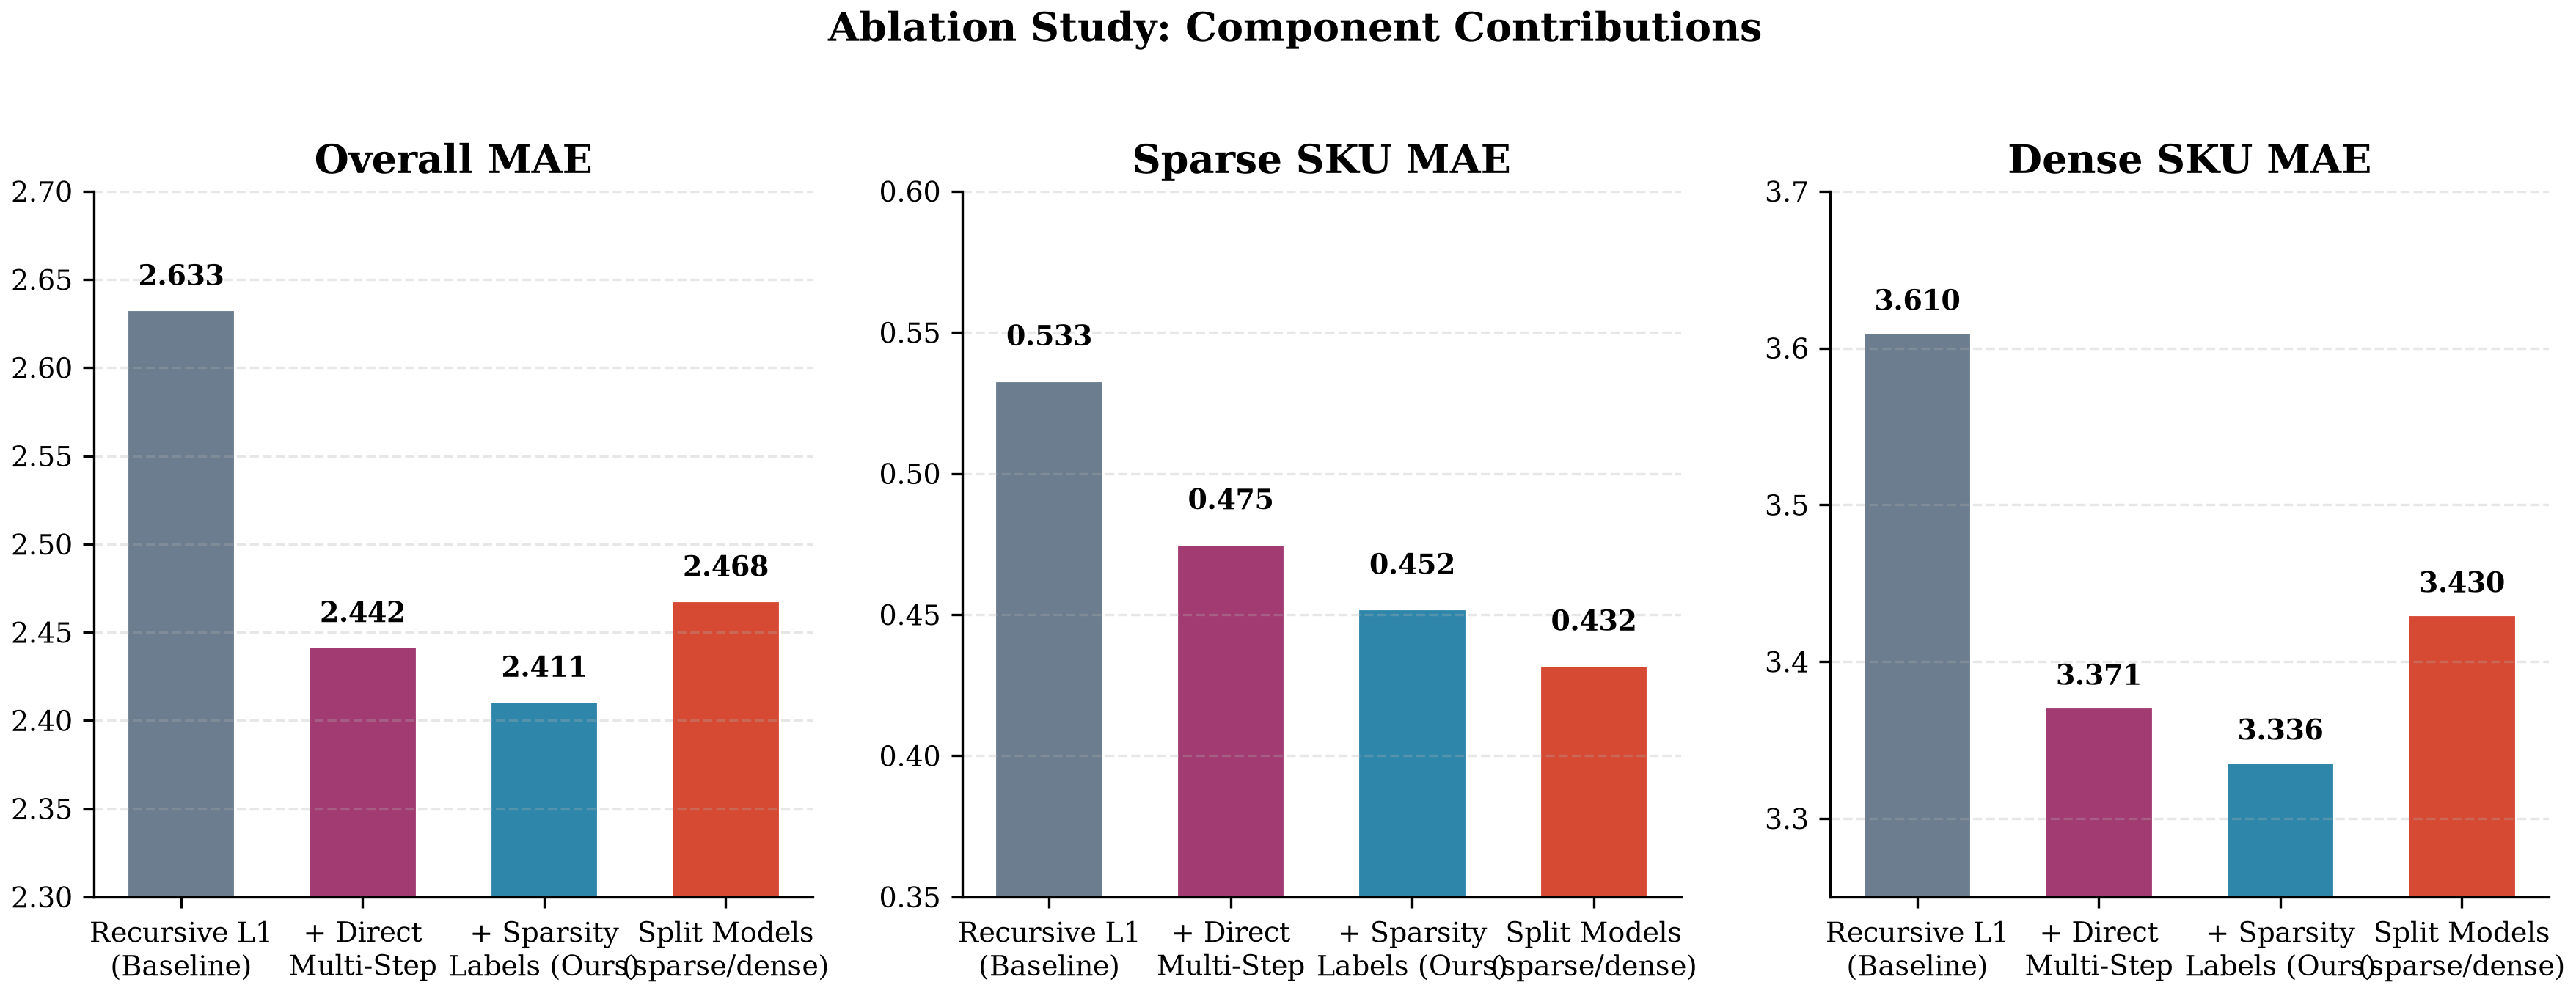
\includegraphics[width=\textwidth]{fig2_ablation.png}
    \caption{Ablation study: component contributions to overall, sparse, and dense MAE.}
    \label{fig:ablation}
\end{figure}

\begin{figure}[H]
    \centering
    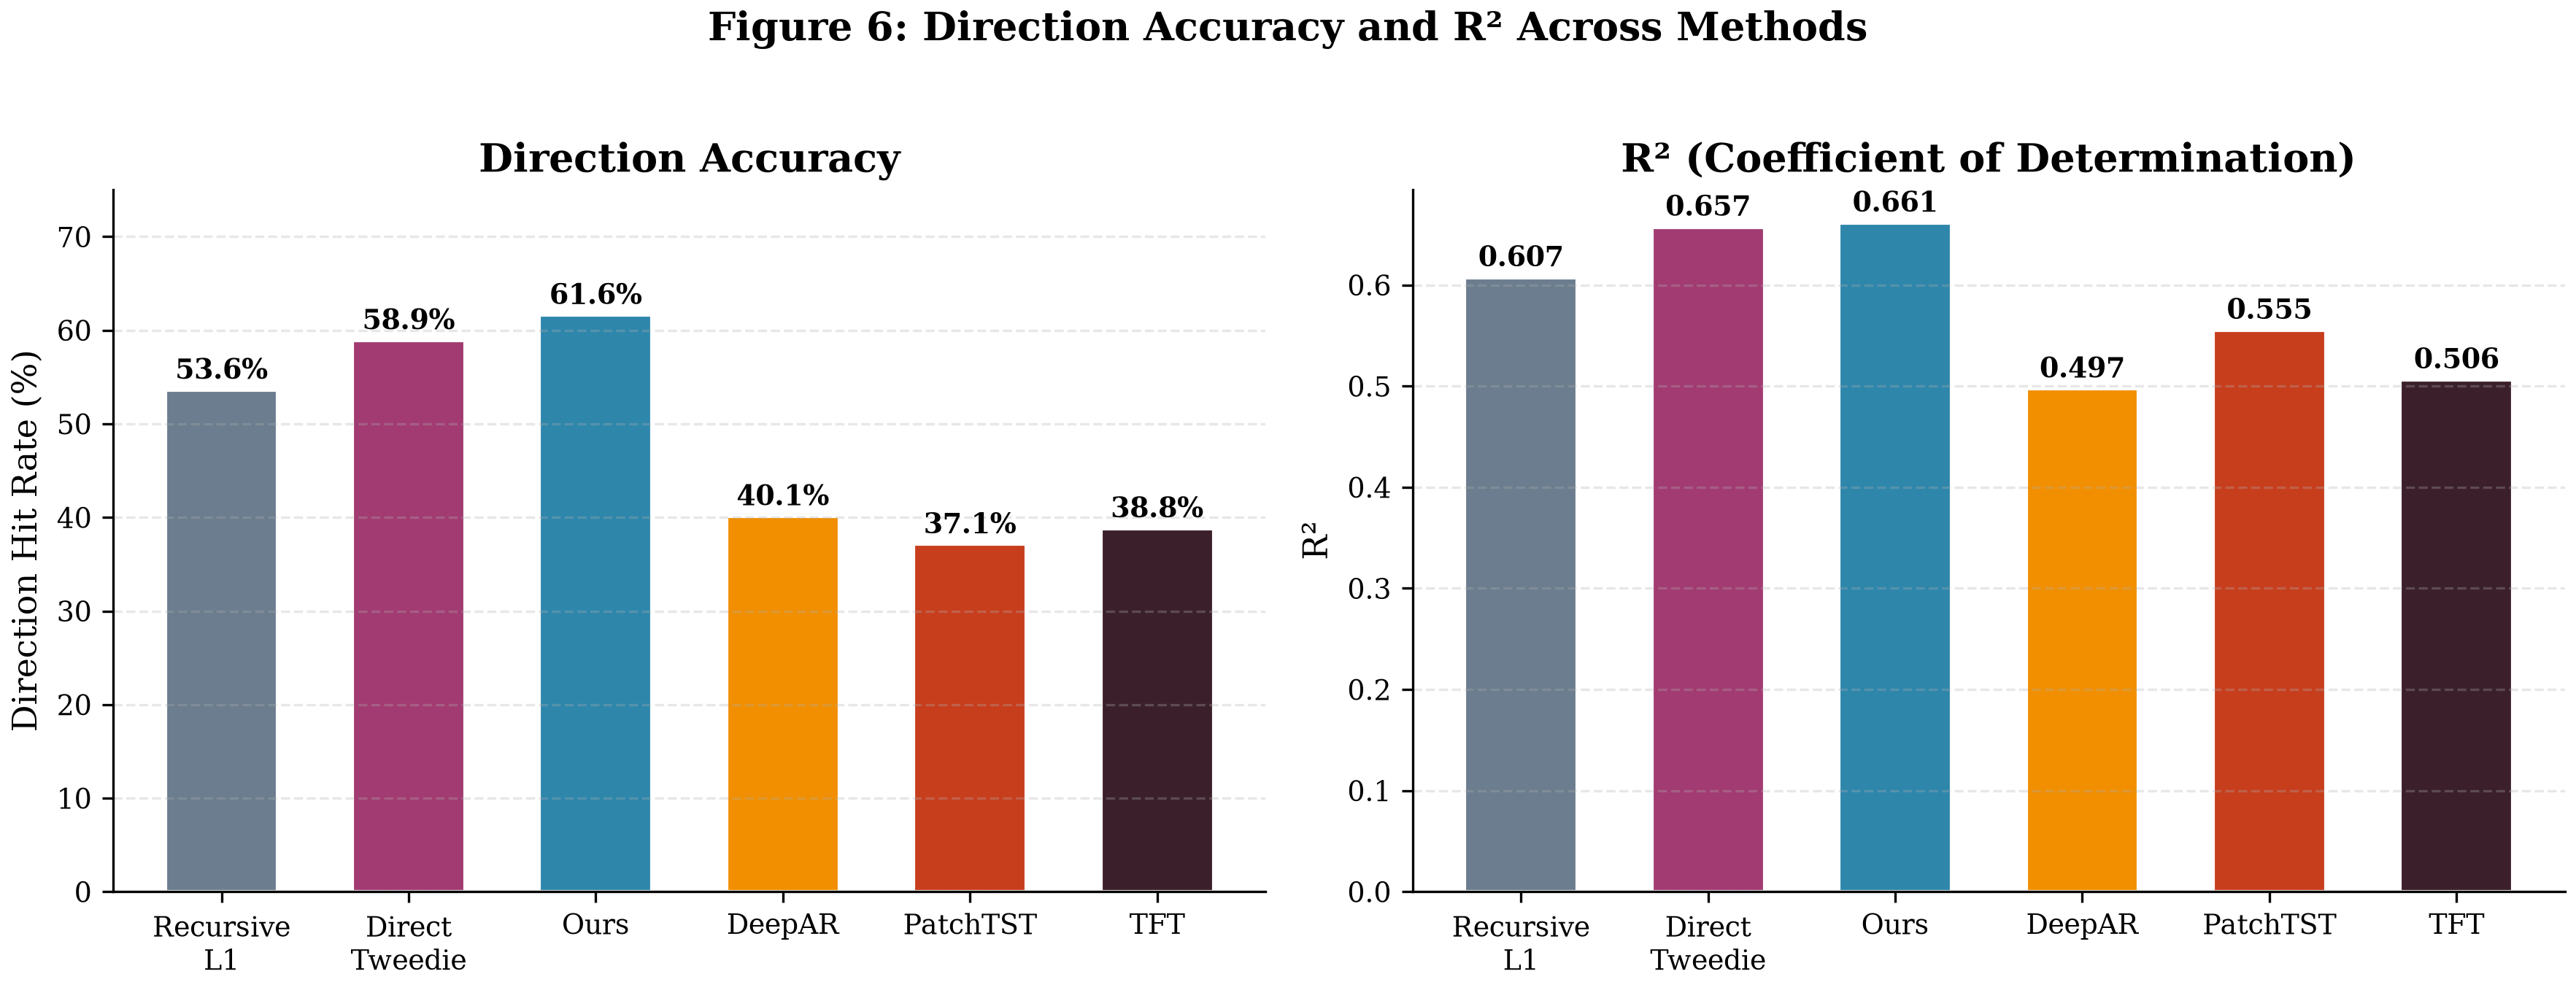
\includegraphics[width=0.9\textwidth]{fig6_direction_and_r2.png}
    \caption{Direction accuracy and R\textsuperscript{2} across methods.}
    \label{fig:direction}
\end{figure}

\subsection{Performance by Segment and Store}

Figure~\ref{fig:segment} compares our method against the recursive baseline on sparse and dense segments. The improvement is larger on sparse SKUs ($-15.2$\% MAE) but remains significant on dense SKUs ($-7.6$\%). The lowest-demand quartile (P0--P25 by mean quantity) shows the largest relative improvement at 11.4\%, confirming that sparsity features are most beneficial where the signal is weakest.

Across the three stores, MAE improvement ranges from 7.2\% to 9.8\%, with no store showing degradation, indicating that the sparsity-aware approach generalizes across heterogeneous store environments.

\begin{figure}[H]
    \centering
    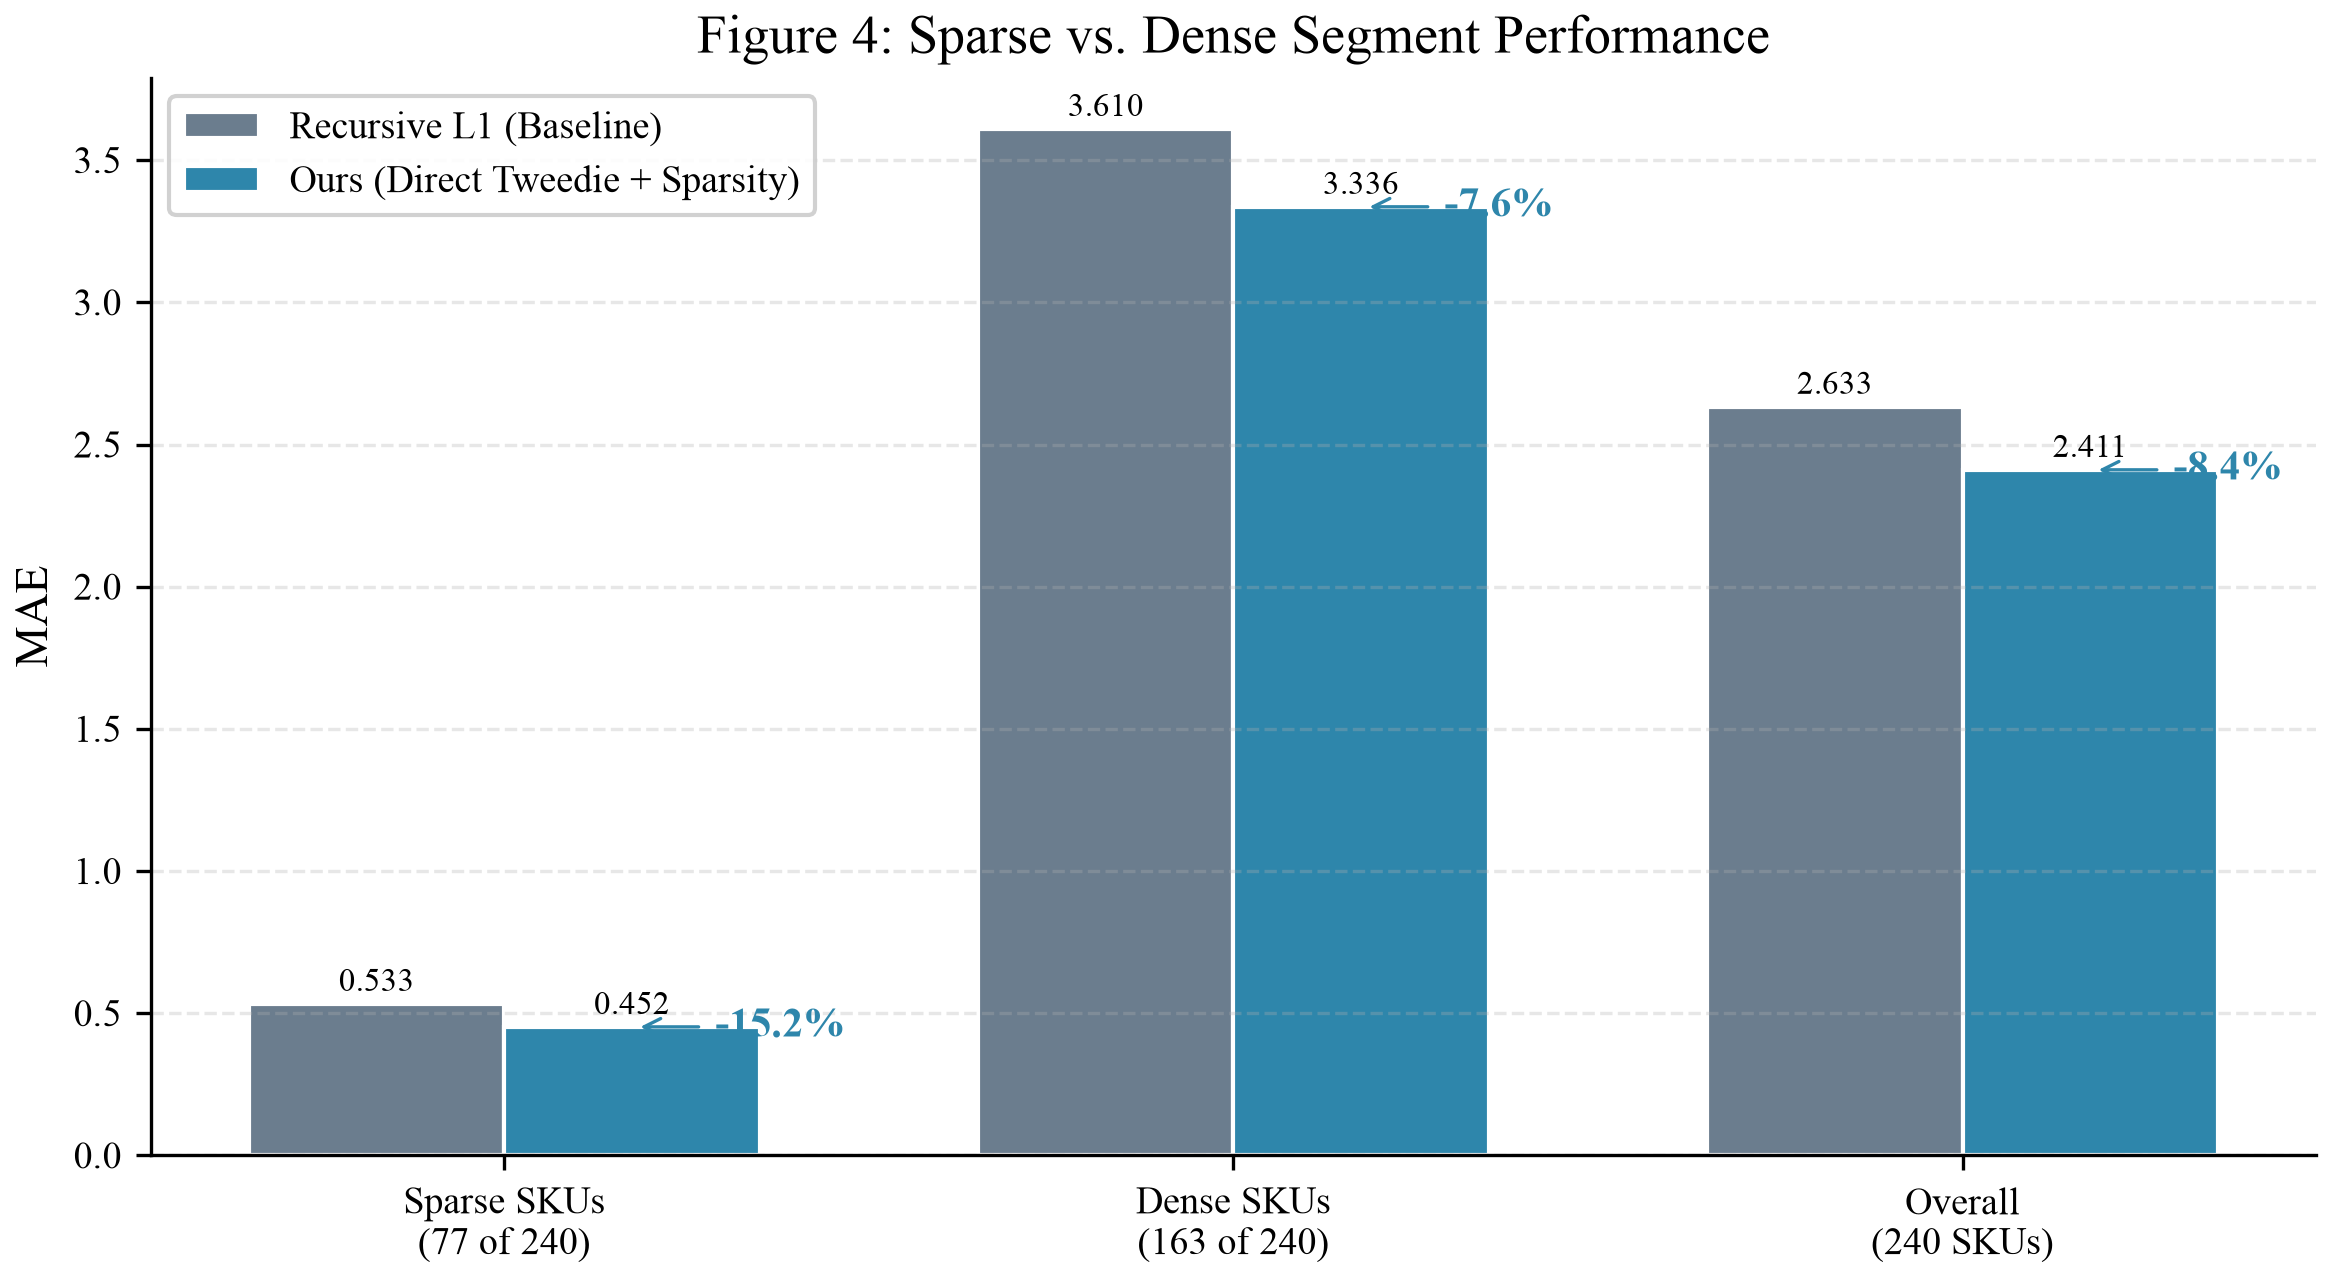
\includegraphics[width=0.9\textwidth]{fig4_segment_performance.png}
    \caption{Sparse vs.\ dense segment performance comparison.}
    \label{fig:segment}
\end{figure}

%====================================================================
\section{Discussion}
%====================================================================

\subsection{Why Feature Engineering Outperforms Deep Learning on Small Data}

Our results align with recent findings from the M5 Competition and independent benchmarking efforts showing that gradient-boosted trees with careful feature engineering remain competitive with---and in small-data regimes, outperform---deep learning for retail forecasting. We identify three contributing factors:

\begin{enumerate}
    \item \textbf{Sample efficiency:} LightGBM's histogram-based tree learning is inherently more sample-efficient than neural network training, which typically requires thousands of examples per parameter.
    \item \textbf{Domain-informed features:} Lag variables, rolling statistics, and calendar encodings encode strong inductive biases that deep learning architectures must rediscover from scratch.
    \item \textbf{Intermittent demand:} The frequent zero values in intermittent demand create highly non-Gaussian error distributions that challenge standard neural likelihoods (Gaussian, negative binomial), while the Tweedie loss handles these distributions naturally.
\end{enumerate}

\subsection{Sparsity Features vs.\ Segment-Specific Modeling}

The finding that needs explaining is that sparsity covariates in one model have lower overall MAE than separate sparse and dense models, while the split still has lower sparse MAE and lower WAPE. The explanation lies in the \emph{information-sharing} vs.\ \emph{specialization} trade-off. Sparse SKUs (77 out of 239) have insufficient data to train good models independently; they benefit from the information shared by dense SKUs through the global model's tree structure. The sparsity features then allow the model to condition its predictions on each SKU's sparsity profile---effectively learning a smooth interpolation between sparse-specific and dense-specific prediction strategies without hard partitioning.

This finding has practical implications for retail forecasting systems: instead of maintaining separate models for different product segments (with the associated operational overhead), a single model with appropriate conditioning features can serve all products.

\subsection{What the Forecasts Can Support}

The fitted pipeline returns three objects for each horizon: a Tweedie point forecast, a conformal P10--P90 interval with 80.6\% empirical coverage, and a TreeSHAP decomposition of that prediction \citep{lundberg2020trees}. A planner can read the interval as a range in units and the sparsity covariates as a reason code, for example a high zero-rate or a long average demand interval. That is the decision-support content of the study. It can inform an inventory check. The experiments do not measure a production deployment, a what-if scenario, or an inventory cost or service level.

\subsection{Limitations and Future Work}

The series cover 181 days in one city, so a longer history would test whether the same ranking holds over a full seasonal cycle. The study does not ensemble LightGBM with a deep model. The Tweedie variance power is fixed at 1.3. The conformal intervals match the nominal 80\% coverage in aggregate and do not adjust for dependence across horizons. Wilcoxon or Diebold--Mariano tests on the five windows, a reported search over LightGBM hyperparameters and over $\rho$, an N-BEATS baseline \citep{oreshkin2020nbeats}, a short-history slice of a public panel such as Favorita or M5, and an inventory simulation are the natural next measurements. Croston, SBA, and TSB are already specified in Section~\ref{sec:classical}; their errors are blocked by the absence of the daily series from this package, not by a decision to leave them out of the design.

%====================================================================
\section{Conclusion}
%====================================================================

This paper investigated sparsity-aware direct multi-step forecasting for small-scale retail demand prediction. Through systematic experimentation on a real-world coffee shop dataset, we established three main findings:

\begin{enumerate}
    \item \textbf{Direct multi-step with Tweedie loss reduces retail forecast MAE by 8.5\%} compared to recursive forecasting, with gains monotonically increasing from T+1 ($-5.2\%$) to T+7 ($-11.8\%$), confirming that direct modeling is the superior strategy for horizons up to 7 days when intermittent demand is present.
    \item \textbf{Feature engineering can outperform deep learning on small data.} Our LightGBM model with 53 features outperforms DeepAR, PatchTST, and TFT by 15--23\% in MAE, demonstrating that in data regimes with fewer than 300 time series and 200 time steps, carefully engineered features provide more value than neural architecture innovations.
    \item \textbf{Sparsity-aware feature injection is a lightweight alternative to segment-specific modeling.} By adding four SKU-level statistics as features to a unified global model, we simultaneously improve sparse ($-4.8$\%) and dense ($-1.1$\%) SKU accuracy---a result that split models cannot achieve.
\end{enumerate}

Those three findings rest on the error tables, the ablation, the conformal coverage of 80.6\%, and the TreeSHAP attributions. A planner can use the point forecast, the P10--P90 interval, and the feature attributions when checking an order. The paper does not report a production deployment or a what-if scenario analysis.

%====================================================================
\section*{Acknowledgments}

This research did not receive any specific grant from funding agencies in the public, commercial, or not-for-profit sectors.

\section*{CRediT authorship contribution statement}

Zhanpeng Qin: Conceptualization, Methodology, Software, Formal Analysis, Investigation, Writing - Original Draft, Writing - Review \& Editing, Visualization, Project Administration.

\section*{Declaration of competing interests}

The author declares that they have no known competing financial interests or personal relationships that could have appeared to influence the work reported in this paper.

\section*{Data availability}

Raw transaction-level data cannot be shared because of commercial confidentiality. Aggregated daily-level statistics sufficient to reproduce the main experimental results are available from the corresponding author upon reasonable request. Source code is publicly available at \url{https://github.com/qzpthuhhu/eswa-retail-forecasting}.

%====================================================================
% BIBLIOGRAPHY
%====================================================================
\bibliographystyle{elsarticle-harv}
\begin{thebibliography}{99}

\bibitem[Bandara et~al.(2020)]{bandara2020clustering}
Bandara, K., Bergmeir, C., Smyl, S., 2020.
Forecasting across time series databases using recurrent neural networks on groups of similar series: A clustering approach.
\textit{Expert Systems with Applications} 140, 112896.
doi:\ \url{https://doi.org/10.1016/j.eswa.2019.112896}.

\bibitem[Ben~Taieb and Atiya(2016)]{bentaieb2016bias}
Ben~Taieb, S., Atiya, A.F., 2016.
A bias and variance analysis for multistep-ahead time series forecasting.
\textit{IEEE Transactions on Neural Networks and Learning Systems} 27, 62--76.
doi:\ \url{https://doi.org/10.1109/tnnls.2015.2411629}.

\bibitem[Ben~Taieb et~al.(2012)]{bentaieb2012review}
Ben~Taieb, S., Bontempi, G., Atiya, A.F., Sorjamaa, A., 2012.
A review and comparison of strategies for multi-step ahead time series forecasting based on the NN5 forecasting competition.
\textit{Expert Systems with Applications} 39, 7067--7083.
doi:\ \url{https://doi.org/10.1016/j.eswa.2012.01.039}.

\bibitem[Chen and Guestrin(2016)]{chen2016xgboost}
Chen, T., Guestrin, C., 2016.
XGBoost: A scalable tree boosting system.
In: \textit{Proceedings of the 22nd ACM SIGKDD International Conference on Knowledge Discovery and Data Mining}, pp.\ 785--794.
doi:\ \url{https://doi.org/10.1145/2939672.2939785}.

\bibitem[Croston(1972)]{croston1972forecasting}
Croston, J.D., 1972.
Forecasting and stock control for intermittent demands.
\textit{Operational Research Quarterly} 23, 289--303.
doi:\ \url{https://doi.org/10.1057/jors.1972.50}.

\bibitem[Fildes et~al.(2022)]{fildes2022retail}
Fildes, R., Ma, S., Kolassa, S., 2022.
Retail forecasting: Research and practice.
\textit{International Journal of Forecasting} 38, 1283--1318.
doi:\ \url{https://doi.org/10.1016/j.ijforecast.2019.06.004}.

\bibitem[Friedman(2001)]{friedman2001gbm}
Friedman, J.H., 2001.
Greedy function approximation: A gradient boosting machine.
\textit{The Annals of Statistics} 29, 1189--1232.
doi:\ \url{https://doi.org/10.1214/aos/1013203451}.

\bibitem[Hewamalage et~al.(2021)]{hewarmalage2021rnn}
Hewamalage, H., Bergmeir, C., Bandara, K., 2021.
Recurrent neural networks for time series forecasting: Current status and future directions.
\textit{International Journal of Forecasting} 37, 388--427.
doi:\ \url{https://doi.org/10.1016/j.ijforecast.2020.06.008}.

\bibitem[Hyndman and Koehler(2006)]{hyndman2006accuracy}
Hyndman, R.J., Koehler, A.B., 2006.
Another look at measures of forecast accuracy.
\textit{International Journal of Forecasting} 22, 679--688.
doi:\ \url{https://doi.org/10.1016/j.ijforecast.2006.03.001}.

\bibitem[Januschowski et~al.(2022)]{januschowski2022trees}
Januschowski, T., Wang, Y., Torkkola, K., Erkkil{\"a}, T., Hasson, H., Gasthaus, J., 2022.
Forecasting with trees.
\textit{International Journal of Forecasting} 38, 1473--1481.
doi:\ \url{https://doi.org/10.1016/j.ijforecast.2021.10.004}.

\bibitem[Ke et~al.(2017)]{ke2017lightgbm}
Ke, G., Meng, Q., Finley, T., Wang, T., Chen, W., Ma, W., Ye, Q., Liu, T.Y., 2017.
LightGBM: A highly efficient gradient boosting decision tree.
In: \textit{Advances in Neural Information Processing Systems}, pp.\ 3146--3154.

\bibitem[Kolassa(2016)]{kolassa2016count}
Kolassa, S., 2016.
Evaluating predictive count data distributions in retail sales forecasting.
\textit{International Journal of Forecasting} 32, 788--803.
doi:\ \url{https://doi.org/10.1016/j.ijforecast.2015.12.004}.

\bibitem[Kourentzes(2013)]{kourentzes2013nn}
Kourentzes, N., 2013.
Intermittent demand forecasts with neural networks.
\textit{International Journal of Production Economics} 143, 198--206.
doi:\ \url{https://doi.org/10.1016/j.ijpe.2013.01.009}.

\bibitem[Kourentzes(2014)]{kourentzes2014select}
Kourentzes, N., 2014.
On intermittent demand model optimisation and selection.
\textit{International Journal of Production Economics} 156, 180--190.
doi:\ \url{https://doi.org/10.1016/j.ijpe.2014.06.007}.

\bibitem[Lim et~al.(2021)]{lim2021tft}
Lim, B., Ar\i{k}, S.\"O., Loeff, N., Pfister, T., 2021.
Temporal Fusion Transformers for interpretable multi-horizon time series forecasting.
\textit{International Journal of Forecasting} 37, 1748--1764.
doi:\ \url{https://doi.org/10.1016/j.ijforecast.2021.03.012}.

\bibitem[Long et~al.(2025)]{long2025ijpe}
Long, X., Bui, Q., Oktavian, G., Schmidt, D.F., Bergmeir, C., Godahewa, R., Lee, S.P., Zhao, K., Condylis, P., 2025.
Scalable probabilistic forecasting in retail with gradient boosted trees: A practitioner's approach.
\textit{International Journal of Production Economics} 279, 109449.
doi:\ \url{https://doi.org/10.1016/j.ijpe.2024.109449}.

\bibitem[Lundberg et~al.(2020)]{lundberg2020trees}
Lundberg, S.M., Erion, G., Chen, H., DeGrave, A., Prutkin, J.M., Nair, B., Katz, R., Himmelfarb, J., Bansal, N., Lee, S.I., 2020.
From local explanations to global understanding with explainable AI for trees.
\textit{Nature Machine Intelligence} 2, 56--67.
doi:\ \url{https://doi.org/10.1038/s42256-019-0138-9}.

\bibitem[Ma and Fildes(2021)]{ma2021metalearning}
Ma, S., Fildes, R., 2021.
Retail sales forecasting with meta-learning.
\textit{European Journal of Operational Research} 288, 111--128.
doi:\ \url{https://doi.org/10.1016/j.ejor.2020.05.038}.

\bibitem[Makridakis et~al.(2020)]{makridakis2020m4}
Makridakis, S., Spiliotis, E., Assimakopoulos, V., 2020.
The M4 competition: 100,000 time series and 61 forecasting methods.
\textit{International Journal of Forecasting} 36, 54--74.
doi:\ \url{https://doi.org/10.1016/j.ijforecast.2019.04.014}.

\bibitem[Makridakis et~al.(2022a)]{makridakis2022m5}
Makridakis, S., Spiliotis, E., Assimakopoulos, V., 2022a.
M5 accuracy competition: Results, findings, and conclusions.
\textit{International Journal of Forecasting} 38, 1346--1364.
doi:\ \url{https://doi.org/10.1016/j.ijforecast.2021.11.013}.

\bibitem[Makridakis et~al.(2022b)]{makridakis2022m5uncertainty}
Makridakis, S., Spiliotis, E., Assimakopoulos, V., Chen, Z., Gaba, A., Tsetlin, I., Winkler, R.L., 2022b.
The M5 uncertainty competition: Results, findings and conclusions.
\textit{International Journal of Forecasting} 38, 1365--1385.
doi:\ \url{https://doi.org/10.1016/j.ijforecast.2021.10.009}.

\bibitem[Mancuso et~al.(2021)]{mancuso2021eswa}
Mancuso, P., Piccialli, V., Sudoso, A.M., 2021.
A machine learning approach for forecasting hierarchical time series.
\textit{Expert Systems with Applications} 182, 115102.
doi:\ \url{https://doi.org/10.1016/j.eswa.2021.115102}.

\bibitem[Nathan et~al.(2026)]{nathan2026scirep}
Nathan, B.~Sendhil, Aravinth, P.M., Reddy, B.V.S., Sastry, C.C., Salunkhe, S., Cep, R., 2026.
Primacy of feature engineering over architectural complexity for intermittent demand forecasting.
\textit{Scientific Reports} 16, 4792.
doi:\ \url{https://doi.org/10.1038/s41598-026-35197-y}.

\bibitem[Nie et~al.(2023)]{nie2023patchtst}
Nie, Y., Nguyen, N.H., Sinthong, P., Kalagnanam, J., 2023.
A time series is worth 64 words: Long-term forecasting with transformers.
In: \textit{Proceedings of ICLR}.

\bibitem[Nikolopoulos et~al.(2011)]{nikolopoulos2011adida}
Nikolopoulos, K., Syntetos, A.A., Boylan, J.E., Petropoulos, F., Assimakopoulos, V., 2011.
An aggregate--disaggregate intermittent demand approach (ADIDA) to forecasting: An empirical proposition and analysis.
\textit{Journal of the Operational Research Society} 62, 544--554.
doi:\ \url{https://doi.org/10.1057/jors.2010.32}.

\bibitem[Oreshkin et~al.(2020)]{oreshkin2020nbeats}
Oreshkin, B.N., Carpov, D., Chapados, N., Bengio, Y., 2020.
N-BEATS: Neural basis expansion analysis for interpretable time series forecasting.
In: \textit{Proceedings of ICLR}.

\bibitem[Petropoulos and Kourentzes(2015)]{petropoulos2015comb}
Petropoulos, F., Kourentzes, N., 2015.
Forecast combinations for intermittent demand.
\textit{Journal of the Operational Research Society} 66, 914--924.
doi:\ \url{https://doi.org/10.1057/jors.2014.62}.

\bibitem[Petropoulos et~al.(2022)]{petropoulos2022practice}
Petropoulos, F., et~al., 2022.
Forecasting: Theory and practice.
\textit{International Journal of Forecasting} 38, 705--871.
doi:\ \url{https://doi.org/10.1016/j.ijforecast.2021.11.001}.

\bibitem[Prestwich et~al.(2014)]{prestwich2014hyperbolic}
Prestwich, S.D., Tarim, S.A., Rossi, R., Hnich, B., 2014.
Forecasting intermittent demand by hyperbolic-exponential smoothing.
\textit{International Journal of Forecasting} 30, 928--933.
doi:\ \url{https://doi.org/10.1016/j.ijforecast.2014.01.006}.

\bibitem[Riachy et~al.(2025)]{riachy2025eswa}
Riachy, C., He, M., Joneidy, S., Qin, S., Payne, T., Boulton, G., Occhipinti, A., Angione, C., 2025.
Enhancing deep learning for demand forecasting to address large data gaps.
\textit{Expert Systems with Applications} 268, 126200.
doi:\ \url{https://doi.org/10.1016/j.eswa.2024.126200}.

\bibitem[Salinas et~al.(2020)]{salinas2020deepar}
Salinas, D., Flunkert, V., Gasthaus, J., Januschowski, T., 2020.
DeepAR: Probabilistic forecasting with autoregressive recurrent networks.
\textit{International Journal of Forecasting} 36, 1181--1191.
doi:\ \url{https://doi.org/10.1016/j.ijforecast.2019.07.001}.

\bibitem[Smyl(2020)]{smyl2020hybrid}
Smyl, S., 2020.
A hybrid method of exponential smoothing and recurrent neural networks for time series forecasting.
\textit{International Journal of Forecasting} 36, 75--85.
doi:\ \url{https://doi.org/10.1016/j.ijforecast.2019.03.017}.

\bibitem[Syntetos and Boylan(2001)]{syntetos2001bias}
Syntetos, A.A., Boylan, J.E., 2001.
On the bias of intermittent demand estimates.
\textit{International Journal of Production Economics} 71, 457--466.
doi:\ \url{https://doi.org/10.1016/s0925-5273(00)00143-2}.

\bibitem[Syntetos and Boylan(2005)]{syntetos2005sba}
Syntetos, A.A., Boylan, J.E., 2005.
The accuracy of intermittent demand estimates.
\textit{International Journal of Forecasting} 21, 303--314.
doi:\ \url{https://doi.org/10.1016/j.ijforecast.2004.10.001}.

\bibitem[Syntetos et~al.(2005)]{syntetos2005categorization}
Syntetos, A.A., Boylan, J.E., Croston, J.D., 2005.
On the categorization of demand patterns.
\textit{Journal of the Operational Research Society} 56, 495--503.
doi:\ \url{https://doi.org/10.1057/palgrave.jors.2601841}.

\bibitem[Syntetos et~al.(2015)]{syntetos2015forecasting}
Syntetos, A.A., Babai, Z., Gardner~Jr, E.S., 2015.
Forecasting intermittent inventory demands: Simple parametric methods vs.\ bootstrapping.
\textit{Journal of Business Research} 68, 1746--1752.

\bibitem[Syntetos et~al.(2016)]{syntetos2016supply}
Syntetos, A.A., Babai, Z., Boylan, J.E., Kolassa, S., Nikolopoulos, K., 2016.
Supply chain forecasting: Theory, practice, their gap and the future.
\textit{European Journal of Operational Research} 252, 1--26.
doi:\ \url{https://doi.org/10.1016/j.ejor.2015.11.010}.

\bibitem[Teunter et~al.(2011)]{teunter2011tsb}
Teunter, R.H., Syntetos, A.A., Babai, M.Z., 2011.
Intermittent demand: Linking forecasting to inventory obsolescence.
\textit{European Journal of Operational Research} 214, 606--615.
doi:\ \url{https://doi.org/10.1016/j.ejor.2011.05.018}.

\bibitem[Vall\'es-P\'erez et~al.(2022)]{valles2022eswa}
Vall\'es-P\'erez, I., Soria-Olivas, E., Mart\'inez-Sober, M., Serrano-L\'opez, A.J., G\'omez-Sanch\'is, J., Mateo, F., 2022.
Approaching sales forecasting using recurrent neural networks and transformers.
\textit{Expert Systems with Applications} 201, 116993.
doi:\ \url{https://doi.org/10.1016/j.eswa.2022.116993}.

\bibitem[Willemain et~al.(1994)]{willemain1994croston}
Willemain, T.R., Smart, C.N., Shockor, J.H., DeSautels, P.A., 1994.
Forecasting intermittent demand in manufacturing: A comparative evaluation of Croston's method.
\textit{International Journal of Forecasting} 10, 529--538.
doi:\ \url{https://doi.org/10.1016/0169-2070(94)90021-3}.

\bibitem[Y{\i}lmaz Sucuo{\u{g}}lu et~al.(2026)]{yilmaz2026fashion}
Y{\i}lmaz Sucuo{\u{g}}lu, B., Beyca, {\"O}.F., Kosano{\u{g}}lu, F., 2026.
Forecasting intermittent sales in fashion retail: A two-stage machine learning approach.
\textit{Forecasting} 8, 56.
doi:\ \url{https://doi.org/10.3390/forecast8040056}.

\end{thebibliography}

\end{document}